%%%%%%%%%%%%%%%%%%%%%%%%%%%%%%%%%%%%%%%%%%%%%%%%%%%%%%%%%%%%%%%%%%%%%%%%%%%%%%%%%%%%%%%%%%%%%%%%%%%%%%%
%%													                                                 %%
%% 	                        BAKALÁŘSKÁ PRÁCE 		                                                 %%
%% 				            Michal Kovář			                                                 %%
%%													                                                 %%
%% pro formátování využita šablona: http://geo3.fsv.cvut.cz/kurzy/mod/resource/view.php?id=775     	 %%
%%                                  https://people.fsv.cvut.cz/~soukup/dip/horcickova/horcickova.pdf %%
%%													                                                 %%
%%%%%%%%%%%%%%%%%%%%%%%%%%%%%%%%%%%%%%%%%%%%%%%%%%%%%%%%%%%%%%%%%%%%%%%%%%%%%%%%%%%%%%%%%%%%%%%%%%%%%%% 

\documentclass[
  12pt,         			% Velikost základního písma je 12 bodů
  a4paper,      			% Formát papíru je A4
  oneside,       			% Oboustranný tisk
  pdftex,				    % překlad bude proveden programem 'pdftex' do PDF
  %twoside                % zarovnaní stran pro oboustranný tisk
]{report}       		  % Dokument třídy 'zpráva'

\newcommand{\Fbox}[1]{\fbox{\strut#1}}

\usepackage[czech, english]{babel}	% použití češtiny, angličtiny
\usepackage[utf8]{inputenc}		% Kódování zdrojových souborů je UTF8

\usepackage[square,sort,comma,numbers]{natbib}

\usepackage{caption}
\usepackage{subcaption}
\captionsetup{font=small}
\usepackage{enumitem} 
\setlist{leftmargin=*} % bez odsazení

\makeatletter
\setlength{\@fptop}{0pt}
\setlength{\@fpbot}{0pt plus 1fil}
\makeatletter

\usepackage[dvips]{graphicx}   
\usepackage{color}
\usepackage{transparent}
\usepackage{wrapfig}
\usepackage{float} 

\usepackage{cmap}           
\usepackage[T1]{fontenc}    

\usepackage{textcomp}
\usepackage[compact]{titlesec}
\usepackage{amsmath}
\addtolength{\jot}{1em} 

\usepackage{chngcntr}
\counterwithout{footnote}{chapter}

\usepackage{acronym}

\usepackage[
    unicode,                
    breaklinks=true,        
    hypertexnames=false,
    colorlinks=true, % true for print version
    citecolor=black,
    filecolor=black,
    linkcolor=black,
    urlcolor=black
]{hyperref}         

\usepackage{url}
\usepackage{fancyhdr}
%\usepackage{algorithmic}
\usepackage{algorithm}
\usepackage{algcompatible}
\renewcommand{\ALG@name}{Pseudokód}% Update algorithm name
\def\ALG@name{Pseudokód}


%%%%%%%%%%%%%%%%%%%%%%%%%%%%%%%%%%%%%%%%%%%%%%%%%%%%%%%%%%%%%%%%%%%%%%%%%%%%%%%%%%%%%%%%%%%%%%%%%%%%%%%
%%													                                                 %%
%%                                     úpravy šablony - Michal Kovář                                 %%

% pro spuštění vlny na celý adresář: for /R %i in (*.tex) do vlna.exe "%i"

\usepackage{pdfpages}% pro přidání celé stránky pdf na radu Filipa
\usepackage{dirtree}% pro tvorubu struktury adresáře
\newcommand\dottedline{\leavevmode\cleaders\hbox to 2.9mm{\hfil.\hfil}\hfill\kern0pt}
\usepackage{marvosym}% znak eura a jarního bodu
\usepackage{qrcode} %tvorba QR kodu na který lze i kliknout
\usepackage{tikz}
\usetikzlibrary{shapes.geometric, arrows}
\usepackage{tikz-3dplot}
\usepackage{eurosym}% pro symbol eura
%\usepackage{ragged2e}% pro vyrovnání do bloku příkazem \justifying
\usepackage{listings}%pro psaní kodu
%\usepackage[none]{hyphenat}% na radu od Filipa pro nazalomování slov

% VLNA JE ZKOMPILOVANÁ NA WINDOWS 10
% Pro spuštění na konkrétní soubor je potřeba mít ten soubor a vlnu v jednom adresáři a zadat příkaz: vlna nazev_souboru.tex
% Pro spuštení na všechny tex soubory v adresáři, kde je vlna a i na všechny soubory v podadresáři slouží příkaz: for /R %i in (*.tex) do vlna.exe "%i"



% Definice vlastního příkazu \tg a \cotg
\newcommand{\tg}{\mathrm{tg}}                                                                        %%
\newcommand{\cotg}{\mathrm{cotg}}                                                                    %%
%%%%%%%%%%%%%%%%%%%%%%%%%%%%%%%%%%%%%%%%%%%%%%%%%%%%%%%%%%%%%%%%%%%%%%%%%%%%%%%%%%%%%%%%%%%%%%%%%%%%%%%

\usepackage[
  cvutstyle,          
  bachelor           
]{thesiscvut}


\newif\ifweb
\ifx\ifHtml\undefined % Mimo HTML.
    \webfalse
\else % V HTML.
    \webtrue
\fi 

\renewcommand{\figurename}{Obrázek}
\def\figurename{Obrázek}

%%%%%%%%%%%%%%%%%%%%%%%%%%%%%%%%%%%%%%%%%%%%%%%%%%%%%%%%%%%%%%%%%
%%%%%%%%%%% Definice informací o dokumentu  %%%%%%%%%%%%%%%%%%%%%
%%%%%%%%%%%%%%%%%%%%%%%%%%%%%%%%%%%%%%%%%%%%%%%%%%%%%%%%%%%%%%%%%

%% Název práce
\nazev{Vývoj zařízení pro příjem a záznam koordinovaného času pro účely astronomického měření}
{sdgfdg}%Vývoj zařízení pro záznam času při a astronomickém měření

%Development of a Device for the Reception and Recording of Coordinated Universal Time for Astronomical Measurement Purposes
%Development of devices for receiving and recording coordinated time for astronomical measurement purposes

%% Jméno a příjmení autora
\autor{Michal}{Kovář}

%% Jméno a příjmení vedoucího práce včetně titulů
\garant{Ing.~Zdeněk~Vyskočil,~Ph.D.}

%% Označení programu studia
\programstudia{Geodézie a~kartografie}{}

%% Označení oboru studia
\oborstudia{GEODÉZIE, KARTOGRAFIE A GEOINFORMATIKA}{}

%% Označení ústavu
\ustav{Katedra geomatiky}{}

%% Rok obhajoby
\rok{2024}

%Mesic obhajoby
\mesic{červen}

%% Místo obhajoby
\misto{Praha}

%% Abstrakt
\abstrakt {Tato bakalářská práce se zabývá vývojem zařízení, které je schopné přijímat a zaznamenávat koordinovaný čas (UTC) pro účely astronomického měření v geodézii. Nejprve je popsána teorie časových soustav a teorie astronomického měření, včetně požadavků na přesnost určení času. Následně jsou popsány možnosti příjmu koordinovaného času. Práce dále popisuje jednotlivé komponenty využité pro tvorbu tohoto zařízení. Je popsána konstrukce výsledného zařízení a řídící program, který zařízení ovládá. Na závěr je testována funkčnost zařízení.}{This bachelor’s thesis deals with the development of a device that is able to receive and record Coordinated Universal Time (UTC) for the purposes of astronomical measurements in geodesy. Initially, the theory of time systems and principles of astronomical measurement are described, including the specification of accuracy requirements for time determination. Subsequently, the possibilities for receiving coordinated time are explored. The thesis further describes the individual components used for the creation of this device. It details the construction of the resulting device and the control program that operates it. At the end, the functionality of the device is tested.}

%% Klíčová slova
\klicovaslova
{astronomické měření, astronomický azimut, časové soustavy, UTC, synchronizace času, Arduino, NTP, DCF77, GNSS}
{astronomical measurement, astronomical azimuth, time systems, UTC, time synchronization, Arduino, NTP, DCF77, GNSS}

%%%%%%%%%%%%%%%%%%%%%%%%%%%%%%%%%%%%%%%%%%%%%%%%%%%%%%%%%%%%%%%%%%%%%%%%

%%%%%%%%%%%%%%%%%%%%%%%%%%%%%%%%%%%%%%%%%%%%%%%%%%%%%%%%%%%%%%%%%%%%%%%%
%% Nastavení polí ve Vlastnostech dokumentu PDF
%%%%%%%%%%%%%%%%%%%%%%%%%%%%%%%%%%%%%%%%%%%%%%%%%%%%%%%%%%%%%%%%%%%%%%%%
\nastavenipdf
%%%%%%%%%%%%%%%%%%%%%%%%%%%%%%%%%%%%%%%%%%%%%%%%%%%%%%%%%%%%%%%%%%%%%%%

%%% Začátek dokumentu
\begin{document}

\catcode`\-=12  % pro vypnuti aktivniho znaku '-' pouzivaneho napr. v \cline 

% aktivace záhlaví
\zahlavi

% předefinování vzhledu záhlaví
\renewcommand{\chaptermark}[1]{%
	\markboth{\MakeUppercase
	{%
	\thechapter.%
	\ #1}}{}}

% Vysázení přebalu práce
%\vytvorobalku

% Vysázení titulní stránky práce
\vytvortitulku {}

\stranka{}%
	{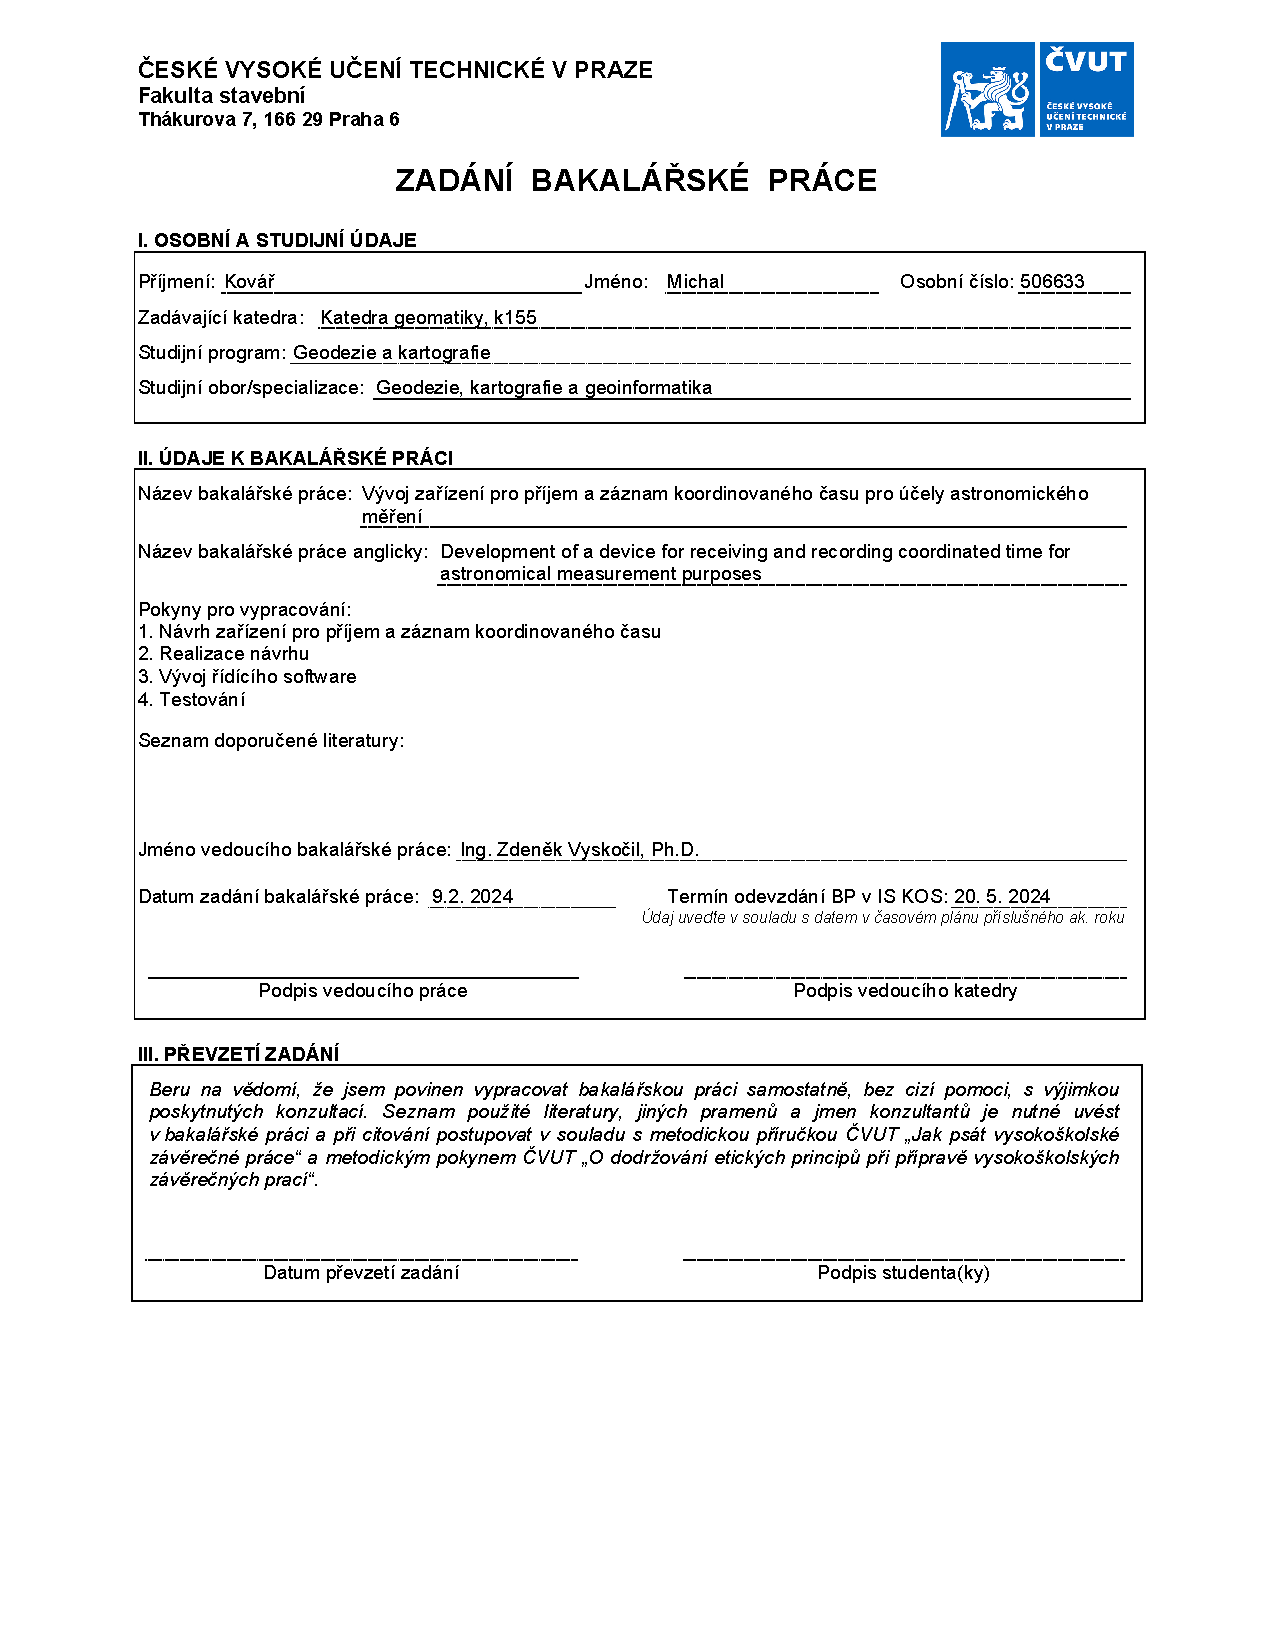
\includepdf[pages=1, offset=15mm -10mm]{./images/zadani/zadani.pdf}
	}

% % Vysázení listu zadani
% \stranka{}%
% 	{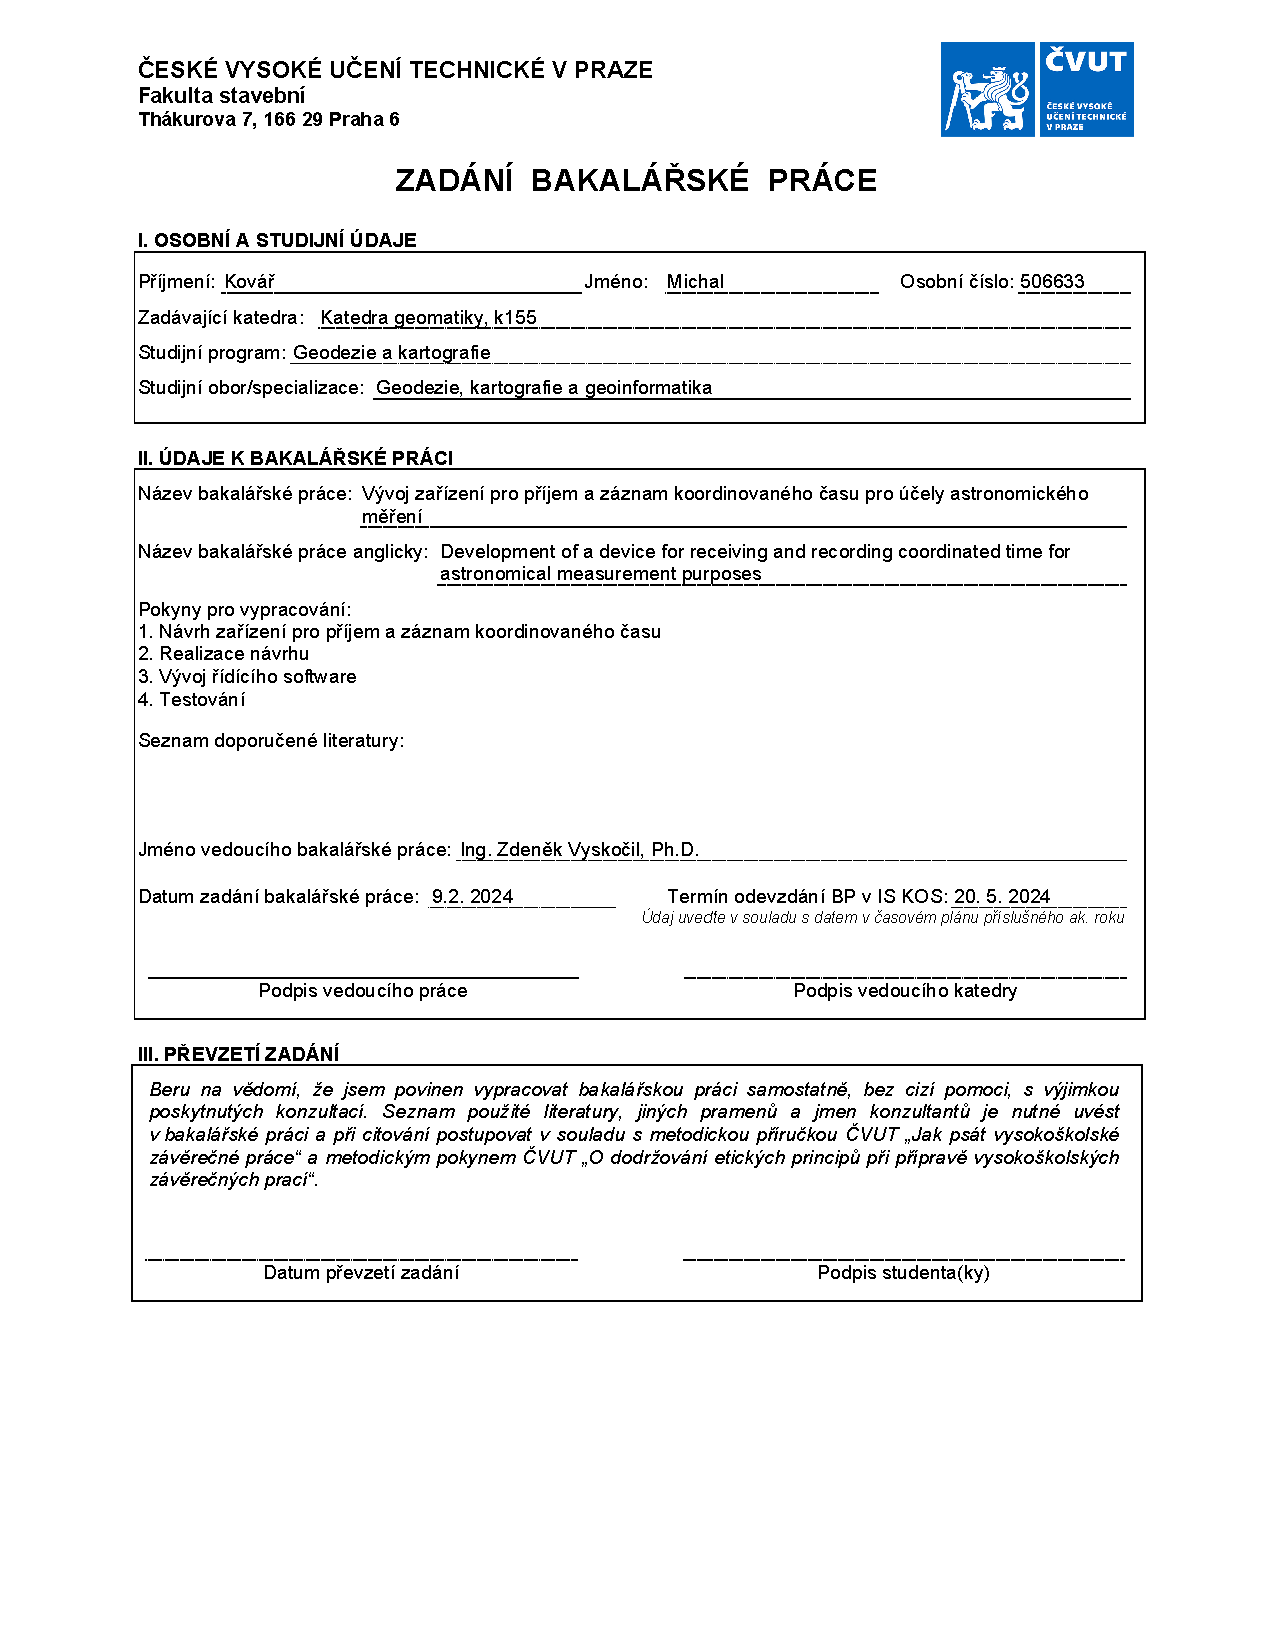
\includegraphics[scale=0.65]{./images/zadani/zadani.pdf}
% 	}%\sffamily\Huge\centering\ }%ZDE VLOŽIT LIST ZADÁNÍ}%
% 	%{\sffamily\centering Z~důvodu správného číslování stránek}

%\stranka{}{    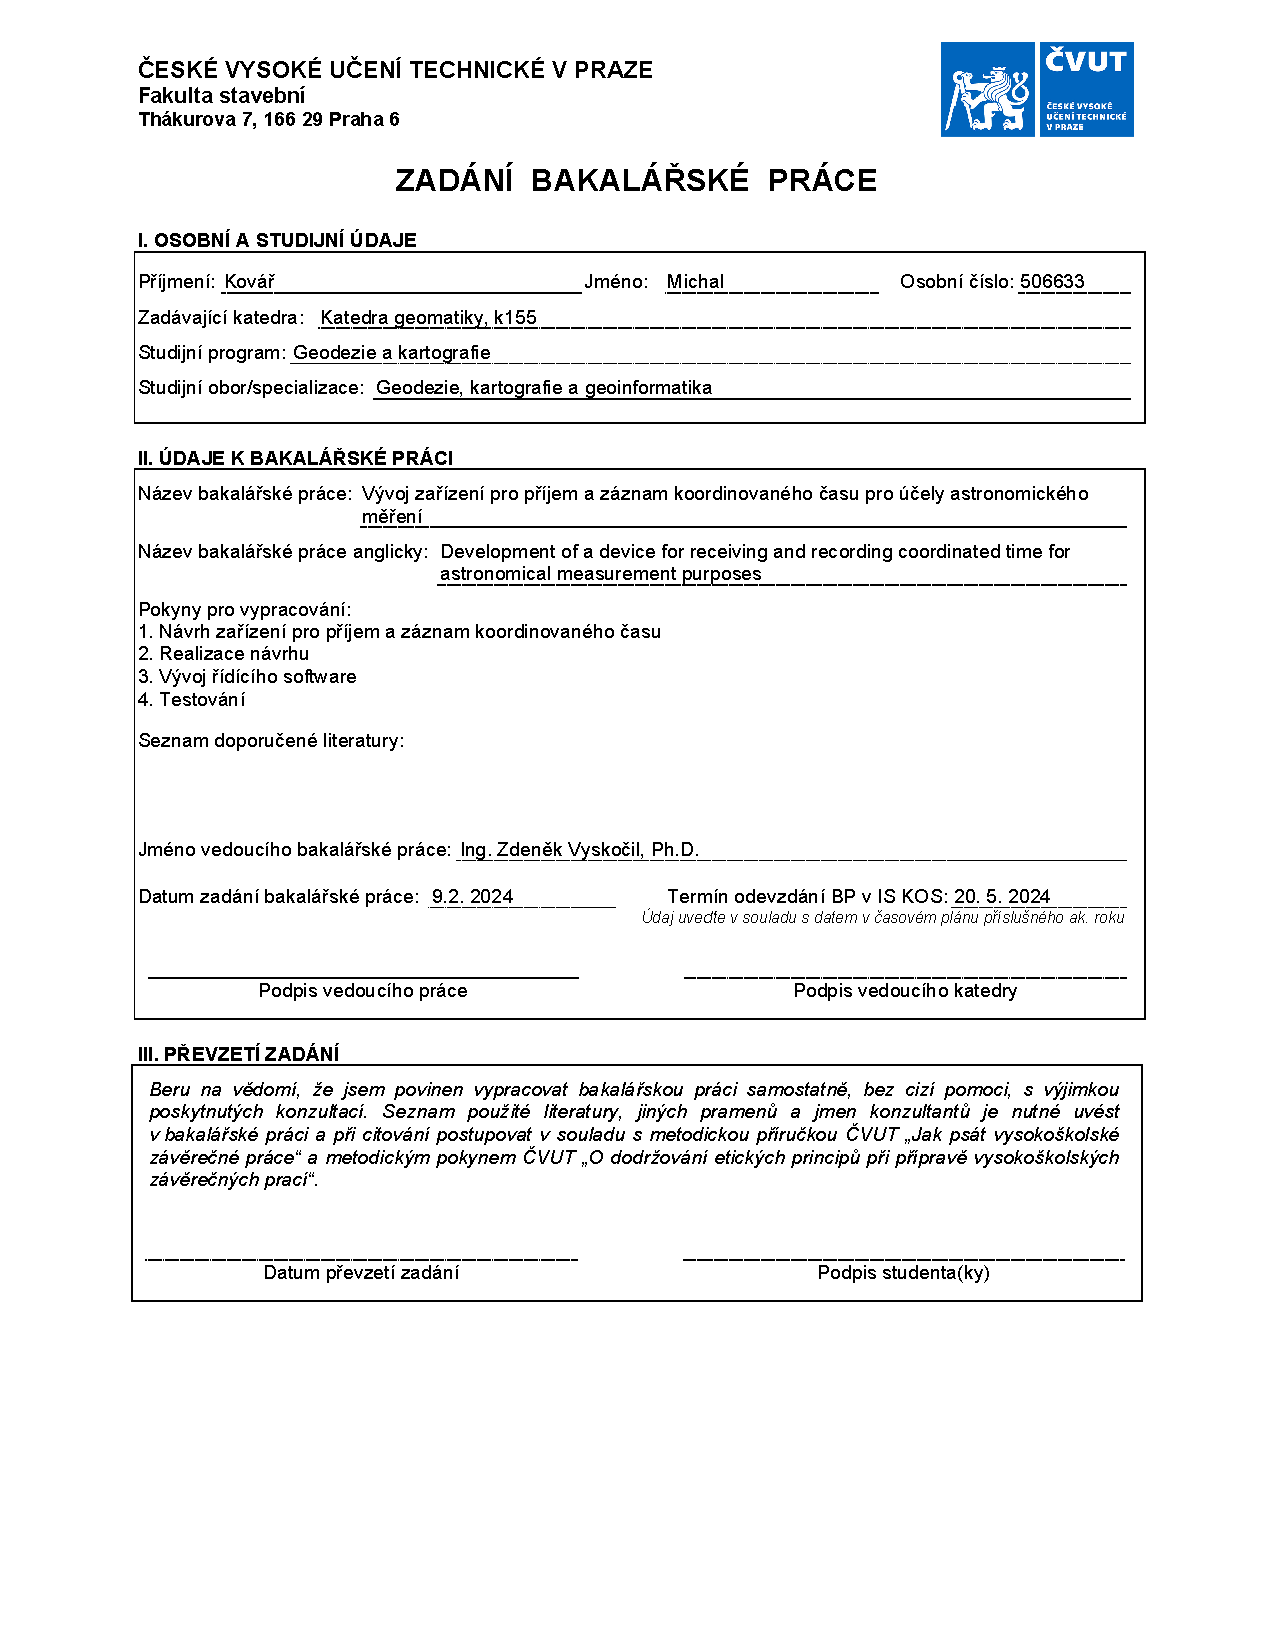
\includepdf[scale=1]{./images/zadani/zadani.pdf}}

% Vysázení stránky s abstraktem
\vytvorabstrakt

% Vysázení prohlaseni o samostatnosti
\vytvorprohlaseni

% Vysázení poděkování
\stranka{%nahore
       }{%uprostred
       }{%dole
       \sffamily
	\begin{flushleft}
		\large
		\MakeUppercase{Poděkování}
	\end{flushleft}
	\vspace{1em}
		%\noindent
	\par\hspace{2ex}
	{Chtěl bych poděkovat Ing.~Zdeňku~Vyskočilovi, Ph.D za jeho ochotu a velké množství cenných rad při vedení této bakalářské práce. Dále bych chtěl poděkovat Ing.~Janu~Holešovskému za rady ohledně průběhu astronomického měření a v neposlední řadě paní Kerstin Eisold za zakoupení součástek, které nebyly v České republice dostupné. Velké poděkování také patří mé rodině za podporu během celého studia.}
}% Kerstin Eisold

% Vysázení obsahu
\obsah

% Vysázení seznamu obrázků
\seznamobrazku

% Vysázení seznamu tabulek
\seznamtabulek

% jednotlivé kapitoly
\chapter{Úvod}
\label{1-uvod}
V~minulosti bylo velmi obtížné určit přesnou polohu objektů na Zemi. Poloha objektů na Zemi byla určována především pomocí geodetické astronomie. Určovaly se astronomické zeměpisné souřadnice (astronomická zeměpisná šířka a astronomická zeměpisná délka) a astronomické azimuty. Během astronomického měření se na rozdíl od klasické geodézie měří na pohyblivé cíle a je tedy nutné zaznamenávat i čas jednotlivých měření. Přesnost určení času má významný vliv na přesnost konkrétních výsledků. 

V~dnešní době byly metody geodetické astronomie z~velké části nahrazeny metodami kosmické geodezie, jako jsou \zk{GNSS} a VLBI. Avšak pro výukové účely má \text{astronomické} měření stále svůj význam. V~současné době se v~rámci výuky \text{teoretické} geodezie zaměřují astronomické azimuty na Slunce. Během tohoto měření se synchro\-nizují stopky (zpravidla na chytrém telefonu) pomocí analogového přijímače signálu DCF77 ručně, a při vlastním měření se záznam provádí druhou osobou na slovní pokyn měřiče. To je příčinou velkých nepřesností v~určení času, které \text{negativně} ovlivňují výsledky celého astronomického měření.

Cílem této práce je navrhnout a vytvořit zařízení schopné přijímat a \text{zaznamenávat} koordinovaný čas pro účely astronomického měření (Astrochronograf). Toto zařízení by mělo být schopno automaticky synchronizovat svůj vnitřní čas, aby \text{nedocházelo} k~chybě z~ruční \text{synchronizace}. Mělo by být jednoduché na ovládání tak, aby mohl astronomické měření snadno provádět i jednotlivec, díky čemuž se eliminuje \text{prodleva} způsobená slovním pokynem. Zařízení by mělo být také schopné \text{informovat} měřiče o~průběhu měření, včetně stavu synchronizace a posledního změřeného času, a umožnit snadný export přehledně zaznamenaných měřených dat.

Výsledné zařízení by mělo být testováno, aby byla ověřena jeho funkčnost. Dále by mělo být zjištěno, jak přesně je zařízení schopno synchronizovat svůj vnitřní čas, jak přesně je schopné zaznamenat měřený čas a jaký vliv má zlepšení určení času na konečné výsledky astronomického měření.
\chapter{Rešerše}
\label{2-reserse}
%https://dspace.cvut.cz/handle/10467/7186
Nepodařilo se dohledat žádnou práci, která by se zabývala explicitně tvorbou \text{zařízení} pro příjem a záznam koordinovaného času pro účely astronomického měření. \text{Podařilo} se však dohledat zdroje, které se zabývají souvisejícími tématy. Geodetickou astro\-nomií se zabývají skripta:
\begin{enumerate}
    \item Geodetická astronomie 10: Toto skriptum bylo vydáno nakladatelstvím ČVUT a zabývá se obecně geodetickou astronomií. Ve skriptu je popsána nauka o~čase, metody geodetické astronomie, přístroje pro astronomické měření včetně přístrojů pro měření času. Skriptum dále obsahuje rozbory přesnosti pro astronomické měření a zmiňuje i požadavky na přesnost určení času \cite{kostelecky_geodeticka_astronomie}.
    \item Geodetická astronomie I. a základy kosmické geodézie: Toto skriptum, bylo \text{vydáno} nakladatelstvím VUTIUM a zabývá se geodetickou astronomií a \text{kosmickou} geodezií. Pro tuto práci je v~něm důležitá především kapitola o~časech a časových systémech \cite{fixel_geodeticka_astronomie}.
\end{enumerate}
Tvorbou zařízení, které umí synchronizovat svůj vnitřní čas se zabývají práce:
\begin{enumerate}
    \item „Časový normál pro centralizovanou správu elektronických hodin“: Tato bakalářská práce se zabývá návrhem a realizací hodinové ústředny, která po zisku časového normálu vzdáleně řídí elektronické hodiny. K~synchronizaci času tato práce využívá tři nezávislé zdroje (DCF77, GPS a NTP server) \cite{pilik_casovy_normal}.
    \item „Elektronické hodiny“: Tato bakalářská práce se zabývá synchronizací času \text{pomocí} DCF77 a GPS přijímače \cite{havlicek_elektronicke_hodiny}.
    \item „Synchronizace času pro odloučená měřící stanoviště“: Tato diplomová práce se zabývá tvorbou zařízení, které pomocí signálu DCF77 synchronizuje čas osobního počítače \cite{zeis_synchronizace_casu}.%Tato práce se zabývá
\end{enumerate}
\chapter{Teorie - Čas}
\label{3-teorie-cas}
Aby bylo možné měřit čas, je potřeba sledovat periodicky se opakující jev. V~minu\-losti se předpokládalo, že rotace Země je rovnoměrná, a tak se pro měření času využívalo měření zdánlivého pohybu nebeských objektů, který je daný rotací Země kolem své osy. Časy vycházející z~rotace Země se nazývají rotační časy. \text{Vzhledem} k~nerovnoměrné rotaci Země, způsobené vlivem precese a nutace, bylo potřeba \text{definovat} čas přesněji. K~tomu se využívají fyzikálně definované časy, které \text{nejsou} navázané na rotaci Země \cite{fixel_geodeticka_astronomie}.

\section{Rotační časy}
Všechny rotační časy jsou odvozené od nerovnoměrné rotace Země a jsou tedy také nerovnoměrné. Rotační časy lze dělit na místní a světové. Místní časy se \text{vztahují} k~astronomické zeměpisné délce pozorovatele \(\lambda\). Světové (greenwichské) jsou \text{vztažené} k~základnímu (greenwichskému) poledníku. Podle toho, zda rotační časy vychází ze zdánlivého pohybu jarního bodu {\Aries} nebo Slunce, je lze dále dělit na časy hvězdné a časy sluneční \cite{kostelecky_geodeticka_astronomie}.

\subsection{Rotační časy hvězdné}%%% nutný přeformulovat
Hvězdné časy jsou definovány jako hodinový úhel jarního bodu \textbf{\Aries}. %, což je úhel mezi směrem k jarnímu bodu \textbf{\Aries} a poledníkem měřený v rovině rovníku.
Světové hvězdné časy jsou vztaženy k~základnímu (Greenwichskému) poledníku a jsou tedy \text{definovány} jako úhel, který je měřený mezi směrem k~jarnímu bodu \textbf{\Aries} a základním \text{poledníkem} \text{v~rovině} rovníku. Místní hvězdné časy jsou definovány analogicky, avšak namísto k~základnímu poledníku se vztahují k~místnímu poledníku. Hvězdný den je \text{definovaný} jako časový interval mezi dvěma po sobě jdoucími horními kulminacemi jarního bodu. Dále lze hvězdné časy dělit na pravé a střední. Pravé hvězdné časy jsou \text{vztaženy} k~pravému jarnímu bodu a jsou ovlivněny precesí i nutací. Střední hvězdné časy jsou vztažené ke střednímu jarnímu bodu a jsou ovlivněné pouze \text{precesí}. Rozdíl pravého místního hvězdného času \(s\) a pravého světového hvězdného času \(S\) je \text{totožný}, jako rozdíl středního místního hvězdného času \(\overline{s}\) a středního \text{světového} \text{hvězdného} času \(\overline{S}\). Tento rozdíl je zároveň roven astronomické zeměpisné šířce \text{místního} \text{poledníku} \(\lambda\) \cite{kostelecky_geodeticka_astronomie}.
\begin{equation}
    s-S=\overline{s}-\overline{S}=\lambda
\end{equation}

\subsection{Rotační časy sluneční}
Smysl zavedení slunečních časů spočívá v~tom, že sluneční časy korespondují s~naším vnímáním světla a tmy. Sluneční den je definován jako časový interval mezi dvěma po sobě jdoucími dolními kulminacemi Slunce. V~důsledku rotace Země kolem Slunce urazí Země každý den v~rovině ekliptiky více než 1°, což mění směr ke Slunci a způsobuje, že sluneční den je zhruba o~4 minuty delší, než hvězdný den \cite{fixel_geodeticka_astronomie}. Sluneční časy lze rozdělit na pravé sluneční časy a střední sluneční časy. Pravé sluneční časy vychází ze zdánlivého pohybu pravého (skutečného) Slunce. Střední sluneční časy vychází z~pohybu fiktivního středního Slunce, které se pohybuje rovnoměrně v~rovině rovníku. Často používaným časovým standardem je střední světový sluneční čas (UT) \cite{kostelecky_geodeticka_astronomie}.

\section{Fyzikální časy}
Fyzikálně definované časy vznikly kvůli nedostatečné přesnosti rotačních časů, způ\-sobené nerovnoměrnou rotací Země. Pro dosažení vyšší přesnosti při určování času je zapotřebí měřit stabilnější, periodicky se opakující jev. V~praxi se nejčastěji využívají hodiny, které jsou založené na měření kmitání atomu cesia. Tyto hodiny se nazývají cesiové atomové hodiny. Z~měření kmitů atomu cesia vychází atomová sekunda, která je základní jednotkou času podle mezinárodního systému jednotek (SI) \cite{kostelecky_geodeticka_astronomie}.

\section{Časové soustavy}%https://lweb.cfa.harvard.edu/ jzhao/times.html#ert
Jelikož je čas odvozený z~rotace Země nerovnoměrný, tak mezinárodní časová služba (BIH) zavedla soustavu světových časů \cite{fixel_geodeticka_astronomie}.

\subsection{Univerzální čas UT0}
Jde o~střední světový sluneční čas (UT), který je vázaný k~místu měření, jelikož je ovlivňován pohybem pólu vzhledem k~danému místu měření \cite{kostelecky_geodeticka_astronomie}.

\subsection{Univerzální čas UT1}
Nerovnoměrnosti v~čase UT0, způsobené kolísáním pravého pólu, jsou v~čase UT1 eliminovány zavedením redukce na střední polohu pólu \(\Delta\lambda_p\) \cite{kostelecky_geodeticka_astronomie}.
\begin{equation}
    UT1=UT0-\Delta\lambda_p
\end{equation}

\subsection{Mezinárodní Atomový čas (TAI)}
Mezinárodní atomový čas (\zk{TAI}, Temps Atomique International) je získán prostřednictvím měření času množstvím nejpřesnějších atomových hodin po celém světě. Časy jednotlivých hodin se liší vlivem systematických chyb a vlivem relativistic\-kých efektů. Po zavedení oprav pro každé atomové hodiny, je \zkratka{TAI} získán jako vážený průměr časů všech zapojených hodin \cite{kostelecky_geodeticka_astronomie} \cite{fixel_geodeticka_astronomie}. Z~\zk{TAI} vychází i GPS čas, který byl zvolen tak, aby se rovnal času \zk{UTC} v~epoše GPS 6. ledna 1980 \cite{kostelecky_glob_poloh_sourad_syst_skripta}. Vztah mezi \zk{TAI} a GPS časem je:
\begin{equation}
    GPS=TAI -19~s
\end{equation}

\subsection{Univerzální koordinovaný čas (UTC)}% opravit nezmiňovat lidi
Jelikož \zk{TAI} není vázaný na rotaci Země a UT1 je nerovnoměrný, byl zaveden \zkratka{UTC}. Ten vychází z~\zk{TAI}, ale je uměle udržován v~blízkosti rotačního času UT1. Délka sekundy TAI i \zk{UTC} je shodná. Vlivem nerovnoměrné rotace Země se přidává přestupná sekunda, která udržuje čas \zk{UTC} v~blízkosti UT1. Rozdíl mezi \zk{UTC} a UT1 je nazýván DUT1 a nikdy nepřesáhne hodnotu ±0,9s. Rozdíl mezi \zk{TAI} a \zk{UTC} je počet přestupných sekund n \cite{kostelecky_geodeticka_astronomie}.
\begin{equation}
    DUT1=UT1-UTC
\end{equation}
\begin{equation}
    n = TAI - UTC
\end{equation}
UTC se běžně používá jako občanský čas. Vychází z~něj i pásmové varianty SEČ a SELČ, které vznikají přičtením jedné, respektive dvou hodin. UTC slouží také pro tvorbu rádiových časových signálů \cite{kostelecky_geodeticka_astronomie}.
\chapter{Teorie - Astronomické měření}
\label{3-teorie-astronomickeho-mereni}
Astronomické měření bylo na našem území prováděno od roku 1863 do roku 1974. Metody měření se v~průběhu času měnily v~závislosti na aktuálním vědeckém poznání a na přesnosti, s~jakou bylo možno určovat čas. Například měření zeměpisné délky vztažené k~základnímu poledníku byla započata až roku 1927, díky existenci rádiových časových signálů. Astronomické měření bylo prováděno především v~rámci astronomicko-geodetické sítě (AGS). Body, u~nichž byly určeny astronomické země\-pisné souřadnice a astronomický azimut, se nazývají Laplaceovy body \cite{kostelecky_geodeticka_astronomie}.

\section{Astronomické azimuty}
V~rámci výuky Teoretické geodézie na FSv ČVUT se měří pouze astronomické \text{azimuty} Slunce metodou určení hodinového úhlu, a tak zde bude zmíněn pouze požadavek přesnosti určení času pro toto měření. Výpočet astronomického azimutu vychází se vztahu:

\begin{equation}    
\tg{(A)} = \frac{\sin(t)}{\sin(\varphi) \cdot \cos(t) - \cos(\varphi) \cdot \tg(\delta)}
\end{equation}

kde \(\delta\) je deklinace Slunce a lze ji zjistit například z~astronomických tabulek\\
a \(t\) je hodinový úhel získaný ze vztahu:

\begin{equation}
    t = S+\lambda-\alpha
\end{equation}

kde \(\alpha\) je rektascenze Slunce a lze ji zjistit například z~astronomických tabulek\\

\(S\) je pravý světový hvězdný čas, který je ovlivněn precesí i nutací a lze jej \text{dopočítat} z~různých časů pomocí vztahů popsaných v~kapitole 3 \cite{kostelecky_geodeticka_astronomie}. Způsob převodu mezi různými časy je naznačen zde: 

\begin{figure}[H]
    \centering
    \begin{tikzpicture}[node distance=2cm]
        \tikzstyle{startstop} = [rectangle, rounded corners, minimum width=3cm, minimum height=1cm,text centered, draw=black, fill=lightgray!30]
        \tikzstyle{arrow} = [thick,->,>=stealth]
        
        \node (GPST) [startstop] {GPS čas};
        \node (TAI) [startstop, below of=GPST] {TAI};
        \node (UTC) [startstop, below of=TAI] {UTC};
        \node (SECS) [startstop, left of=UTC, xshift=-3cm, anchor=center] {SEČ/SELČ};
        \node (nev) [startstop, right of=UTC, xshift=3cm, anchor=center, fill=white, draw=white] {}; % Neviditelný uzel bílý obrys
        \node (UT1) [startstop, below of=UTC] {UT1};
        \node (S_S0) [startstop, below of=UT1] {S-S0};
        
        \draw [arrow] (GPST) -- node[right] {+19s} (TAI);
        \draw [arrow] (TAI) -- node[right] {-n} (UTC);
        \draw [arrow] (SECS) -- node[above] {-1h/-2h} (UTC);
        %\draw [arrow] (nev) -- (UTC); % Šipka z neviditelného uzlu na UTC
        \draw [arrow] (UTC) -- node[right] {+DUT1} (UT1);
        \draw [arrow] (UT1) -- node[right] {\(\cdot (1+\mu)\)} (S_S0);
    \end{tikzpicture}
    \small
    \\
    *\(S_0\) je světový hvězdný čas pro 0h UT1 [h] v~den pozorováni\\
    *\(\mu\) lze dohledat v~astronomických tabulkách
    \caption{Schéma konverze časových údajů}
\end{figure}


Do výpočtu tedy vstupují zeměpisné souřadnice stanoviska a čas měření na Slunce, zbylé hodnoty lze zjistit z~astronomických tabulek a bulletinu mezinárodní služby IERS. Experimentálním dosazením hodnot do vztahů (4.1) pro zeměpisné souřadnice stanoviska 50° s. š. a 15° v. d. a hodnot vycházejících z~časů UTC lišících se o~1s 0.1s a 0.01s byl orientačně zjištěn vliv chyby v~určení času na výsledný astronomický azimut Slunce.


\begin{table}[H]
    \centering
    \caption{Rozdíly azimutů Slunce v~závislosti na rozdílu časů UTC}
    \begin{tabular}{|c|c|c|}
    \hline
    \( \Delta \) UTC [s] & Rozdíl azimutů ["] & Rozdíl azimutů [\(^{cc}\)] \\
    \hline \hline
    1    & 13.93 & 43.01 \\ \hline
    0.1  &  1.39 & 4.30  \\ \hline
    0.01 &  0.13 & 0.43  \\ \hline
    \end{tabular}
\end{table}

Z~tabulky vyplývá, že aby byla chyba v~určení azimutu Slunce menší než jedna úhlová vteřina, je potřeba určovat čas s~přesností na setiny sekund.
\chapter{Teorie - Možnosti určení času}
\label{4-teorie-urceni-casu}
Existuje mnoho možností, jak synchronizovat čas. Mezi nejběžnější patří synchronizace pomocí internetu, rádiového signálu nebo GNSS přijímače.

\section{Internet}
Na internetu jsou dostupné zdroje poskytující informace o~aktuálním koordinovaném světovém čase UTC. Hlavní výhodou synchronizace času pomocí internetu je její snadná dostupnost. Tato metoda je dostupná celosvětově na všech místech s~připojením k~internetu. Nevýhodou je, že může být přesnost synchronizace času ovlivněna latencí internetového připojení. Nejčastěji se lze setkat s~\zk{API} a \zk{NTP} servery.

\subsection{API}
\zkratka{API} je rozhraní, které slouží pro předávání dat mezi softwarovými aplikacemi.
\zk{API} může být použito k~získání času z~webové služby. Například, World Time API slouží pro získání aktuálního času a poskytuje čas pro konkrétní časová pásma ve tvaru Unixového času, nebo ve tvaru podle ISO8601. Data jsou poskytována ve formátu prostého textu nebo jako JSON \cite{worldtimeapi}.

\subsection{NTP}
\zkratka{NTP} servery jsou nejběžněji využívaným zdrojem pro synchronizaci času přes internet. \zk{NTP} je navržený tak, aby na něj neměla velký vliv proměnlivá latence internetového připojení. K~posílání informací slouží v~\zk{NTP} serverech takzvané packety, které obsahují vždy menší množství dat. K~omezení vlivu latence internetového připojení jsou využívány sofistikované algoritmy, díky nimž se přesnost synchronizace času pohybuje do 10 ms \cite{timetools}. Příkladem NTP serveru je Google Public NTP a NTP Pool \cite{ntppool}.
%https://home.zcu.cz/~poupa/pccas.html
% 50ms je sntp
%klasické ntp je lepší : https://timetoolsltd.com/ntp/ntp-timing-accuracy/

\section{Rádiový signál}
Existují vysílače, které vysílají informace o~čase pomocí radiových vln. Tyto signály jsou obvykle velmi přesné, ale jejich příjem může být ovlivněn atmosférickými podmínkami nebo rušením signálu. Příkladem těchto vysílačů jsou WWVB v~USA, MSF ve Velké Británii a DCF77 v~Německu. V~minulosti existoval v~ČR vysílač OMA 50, který od roku 1995 není v~provozu \cite{vyvoj_hw_poupa}.% seznam vysílačů: https://en.wikipedia.org/wiki/Radio_clock

\subsection{DCF77}
Vzhledem k~omezenému dosahu rádiového signálu má na území ČR smysl uvažovat o~využití pouze signálu DCF77. Vysílač DCF77 vysílá čas vycházející z~měření cesiových atomových hodin Fyzikálně-technického institutu v~Braunschweigu (PTB). Tento vysílač vysílá dlouhovlnné rádiové vlny na kmitočtu 77,5 kHz. Výkon vysílače je 50kW. Vysílač vysílá nepřetržitě od roku 1970 a odstaven je jen velmi výjimečně z~důvodů údržby. Teoretický dosah vysílače je uváděn až 2000 km, což však platí jen za ideálních podmínek. Dosah vysílače i za méně příznivých podmínek je udáván 1100~km, což stále pokrývá celé území České republiky.\cite{ptb_dcf77} Název DCF77 vychází z~označení:
\begin{description}[leftmargin=!,labelwidth=\widthof{\bfseries D --}]
    \item[\textbf{D} --] Deutschland (Německo)
    \item[\textbf{C} --] Označení pásma dlouhých vln
    \item[\textbf{F} --] Frankfurtský region
    \item[\textbf{77} --] Vysílací frekvence (77,5 kHz)
\end{description}

\textbf{Časový kód signálu DCF77:}
Každou minutu vysílač vysílá informaci o~\text{minutě}, hodině, dni v~týdnu, měsíci a roku pomocí amplitudové modulace. Tato \text{informace} platí vždy pro následující minutu \cite{fel_dcf77}. Dále je signál modulován pomocí pseudo\-náhodné fázové modulace, která slouží pro přenos pseudonáhodného šumu, který lze využít pro přesnější určení času \cite{vyvoj_hw_poupa} \cite{ptb_2012}.

\begin{figure}[H]
	\centering
	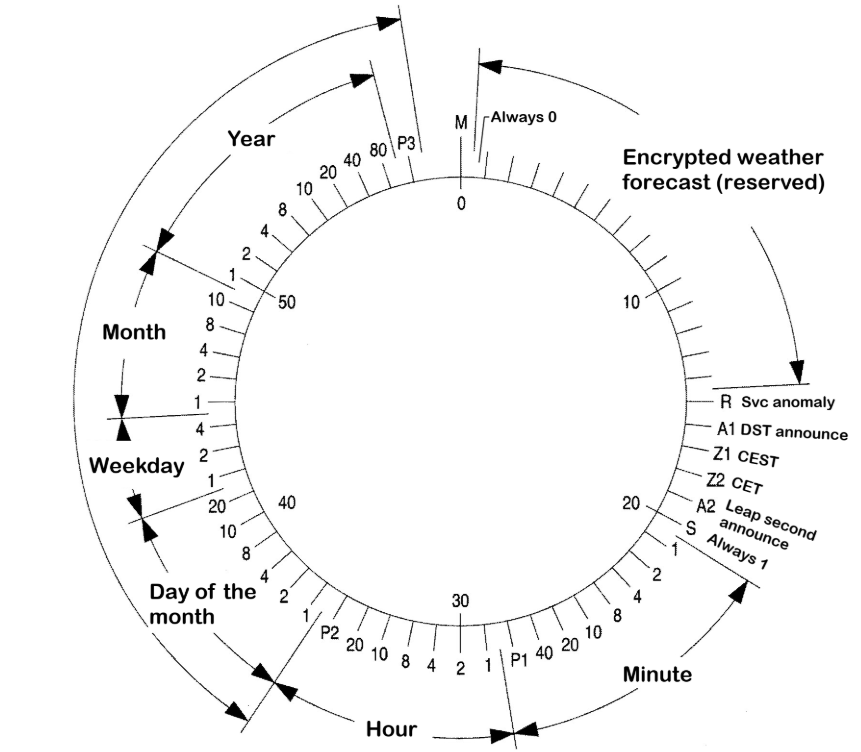
\includegraphics[width=8.4cm]{images/komponenty/schema_DCF77_signalu_lepsi.png}
	\caption{Schéma signálu DCF 77 \cite{fel_dcf77}}
\end{figure}

\textbf{Rušení signálu DCF77:}
Signál DCF77 se šíří ohybem po povrchu Země a odrazem od ionosféry. Odrazy od ionosféry jsou přes den slabé, a proto je signál během dne slabší. Signál DCF77 je rušen z~několika zdrojů. Jedním zdrojem rušení je atmosférický šum způsobený činností ionosféry a může dosahovat velikosti až 80~dB. Atmosférický šum je proměnlivý. Dále může být signál rušen průmyslovou činností, například vlivem vysokonapěťového vedení \cite{vyvoj_hw_andel} \cite{hopf_dcf77}.

\section{GNSS}
Pro určení času lze využít \zkratka{GNSS} jako je GPS, GLONASS nebo Galileo. Družice těchto systémů vysílají časové informace spolu s~navigačními daty. Na satelitech těchto systémů jsou obvykle cesiové atomové hodiny a záložní rubidiové atomové hodiny, které poskytují velmi přesný zdroj času. Signál z těchto družic jsou schopny přijímat GNSS přijímače. Signál je ovšem z~důvodu tranzitní doby opožděn. Pokud přijímač přijímá v~jednu epochu signál alespoň ze čtyř družic, je schopen spočítat opravu hodin přijímače a tím získat svůj přesný čas. Tento čas poskytují GNSS přijímače prostřednictvím NMEA zprávy.

Je potřeba si uvědomit, že například GPS družice pracují v~GPS čase, který je odlišný od času UTC. Součástí NMEA zprávy \$GNZDA je však už čas přepočítaný do UTC \cite{ublox}. Tato metoda poskytuje velmi přesný čas a je dostupná kdekoliv na Zemi, ale vyžaduje přímý výhled na oblohu pro příjem signálů od alespoň čtyř satelitů, aby bylo možné spočítat i opravu hodin přijímače.


\chapter{Vývoj zařízení - Komponenty}
\label{4-vyvoj-zarizeni-komponenty}
\section{Vývojová deska}
Vývojová deska je elektronické zařízení skládající se z~desky plošných spojů, mikro\-kontroléru a k~němu připojených dalších periférií. Mikrokontrolér je malý \text{počítač} na jednom integrovaném obvodu, který může obsahovat jedno nebo více jader \text{procesoru}, paměť pro uložení programu, operační paměť a programovatelné \text{vstupy/výstupy}. Mikrokontrolér neobsahuje operační systém a řídící program na něj bývá nahraný \text{pomocí} integrovaného vývojového prostředí (\zk{IDE}, z~anglického Integrated Develop\-ment Environment). Mikrokontrolér ovládá k~němu připojené periférie a další součástky připojnené k~vývojové desce. Připojením součástek k~vývojové desce lze vytvořit nové elektronické zařízení \cite{dps_vyvojove_desky}.

\subsection{Arduino Uno}
Jako vývojová deska bylo zvoleno Arduino UNO, a to z~důvodu jeho poměrně nízké ceny, velkého množství dostupné dokumentace a kompatibilních součástek. Tato vývojová deska, na které je nahraný řídící program, ovládá všechny ostatní použité komponenty. Nejběžněji se lze setkat s~Arduinem UNO R3, které je \text{založené} na mikrokontroléru ATmega328P od firmy Atmel. Z~důvodu malé kapacity paměti \text{Arduina} UNO R3 bylo využito novější Arduino UNO R4. To je založeno na mikrokontroléru Renesas RA4M1, jenž obsahuje procesor ARM Cortex-M4F. Arduino UNO R4 se vyrábí ve verzích Minima a WiFi. Verze WiFi je zaměřena na IoT aplikace a obsahuje navíc mikrokontrolér ESP32-S3 od firmy Espressif s~integrovaným WiFi a bluetooth low energy (BLE) modulem. Toho lze využít pro připojení k~NTP serveru, nebo odesílání dat \cite{arduino}. Arduino UNO lze pořídit i v~podobě „klonu“, který vyrábí neoficiální výrobce. Tyto „kolny“ bývají obvykle cenově dostupnější než \text{originální desky}.

% https://www.robotikabrno.cz/docs/arduino/Pr%C5%AFvodce-sv%C4%9Btem-Arduina-CZ.pdf

\begin{table}[H]
    \centering
    \caption{Porovnání kapacity paměti Arduina UNO R3 a R4 \cite{arduino}}
    \begin{tabular}{|c|c|c|}
    \hline
    \textbf{Typ paměti} & \textbf{R3} & \textbf{R4}\\
    \hline\hline
    flash  & 32 KB & 256 kB \\ \hline
    SRAM   & 2  KB &  32 kB \\ \hline
    EEPROM & 1  KB &   8 kB \\ \hline
    \end{tabular}\\
\end{table}

\begin{figure}[H]
	\centering
	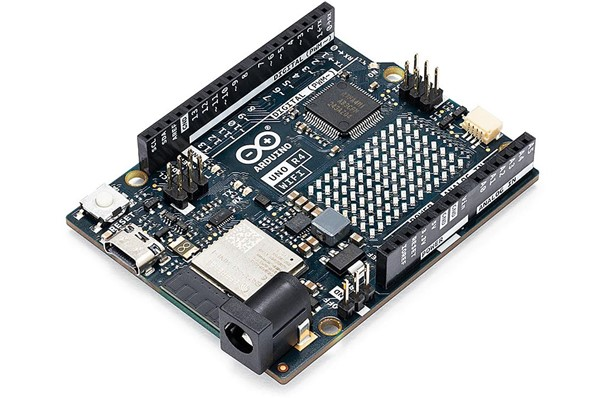
\includegraphics[width=6.5cm]{images/komponenty/UNO_R4.jpg}
	\caption{Arduino UNO R4 ve verzi WiFi \cite{laskakit_web}}
\end{figure}


\subsection{Arduino Mega}
Vzhledem k~nedostatečné kapacitě paměti Arduina UNO R3 se rovněž nabízí možnost využití Arduina Mega. To je založené na mikrokontroléru ATmega2560. Oproti \text{Arduinu} UNO R3 disponuje větší kapacitou paměti, a oproti oběma verzím Arduina UNO i větším množstvím pinů. Nevýhodou Arduina Mega je větší fyzická velikost a bylo tedy využito jen pro testování během vývoje zařízení \cite{arduino}.


\begin{figure}[H]
	\centering
	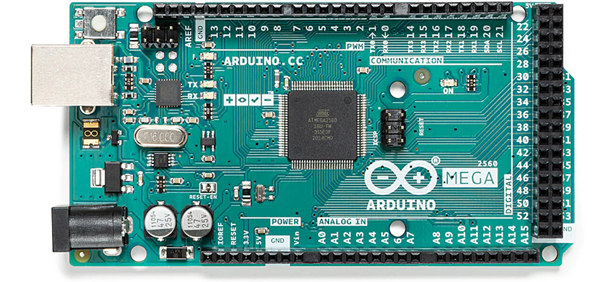
\includegraphics[width=6.5cm]{images/komponenty/mega.png}
	\caption{Arduino Mega \cite{arduino}}
\end{figure}

\section{Přijímač časového signálu}
Existuje několik způsobů, jak synchronizovat čas Arduina s~koordinovaným časem. Jedním z~nich je synchronizace času při nahrávání programu do Arduina. Tato metoda však vyžaduje opakované nahrání programu před každým měřením, aby se interní čas aktualizoval. Tato metoda neumožňuje průběžnou synchronizaci a její přesnost je závislá na přesnosti vnitřního času zařízení z~nějž je program nahráván. Vhodnějšími metodami jsou synchronizace přes internet, využití přijímače DCF77, který přijímá koordinovaný čas pomocí rádiového signálu, nebo využití času z~NMEA zprávy z~GNSS přijímače. Tyto metody poskytují přesnější a průběžnou synchronizaci času bez nutnosti opakovaného nahrávání programu.

\subsection{Přijímač DCF77}
Pro příjem signálu DCF77 je vhodné zvolit anténu, která přijímá především magnetickou složku elektromagnetické vlny, protože elektrická složka vlny je citlivá na výšku antény nad povrchem a bývá výrazně více rušena okolním signálem z~jiných \text{elektronických} zařízení než magnetická složka. Pro příjem magnetické složky signálu lze využít rámovou anténu, která ale mívá poměrně velké rozměry. Obvykle se používá anténa o~průměru 0,5m. Z~důvodu kompaktnosti celého zařízení byla \text{zvolena} feritová anténa. Pokud by signál z~feritové antény nebyl dostatečně silný, je možné pro jeho zesílení přímo na feritovou anténu připojit rámovou anténu s~větším průměrem.

Využitý přijímač se skládá z~feritového jádra, kolem kterého je vinuta cívka a demodulátoru, který slouží k~oddělení modulačního signálu od nosného signálu. Anténa má dvě maxima a dvě minima. Pro příjem maximální intenzity signálu, je vhodné ji umístit kolmo na směr k~vysílači. Pokud by docházelo k~rušení signálu z~jednoho směru, lze to vyřešit tím, že bude anténa natočena minimem ke zdroji rušení \cite{fel_dcf77} \cite{vyvoj_hw_andel}.

\begin{figure}[H]
	\centering
	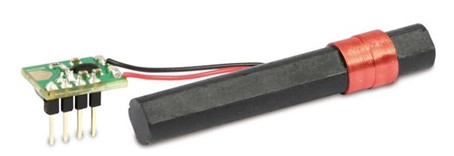
\includegraphics[width=6.1cm]{images/komponenty/DCF77_reciever.jpg}
	\caption{Přijímač radiového signálu DCF77 \cite{dratek_web}}
\end{figure}


\subsection{Přijímač GNSS}
Pro příjem informací o~aktuálním čase lze využít i GNSS přijímač. \text{Astrochrograf} je navržený tak, že má vyvedený pin D0 Arduina, aby k~němu mohl být \text{připojen} \text{libovolný} GNSS přijímač. Pin D0 na Arduinu Uno funguje jako RX pin pro \text{sériovou} komunikaci pomocí UART. GNSS přijímač musí být k~RX pinu Arduina \text{připojen} pomocí svého TX pinu. Přijímač musí poskytovat NMEA zprávu \$GNZDA, která obsahuje informace o~aktuálním čase a zprávu \$GNGGA, která poskytuje informaci o~poloze přijímače. Pro vývoj zařízení byl použit aktuálně dostupný GNSS \text{přijímač} Ublox NEO-M8T, který je schopen přijímat data ze satelitů GPS, GLONASS, Galileo, BeiDou, QZSS a SBAS. Tento přijímač umožňuje i RTK měření. Nevýhodou přijímače je poměrně vysoká cena. Pro určování času lze využít i přijímače s~omeze\-nější funkcionalitou než Ublox NEO-M8T. Například levnější přijímač Ublox NEO-M7M, který přijímá data ze satelitů GPS, GLONASS, Galileo a QZSS. Tento přijímač neumožňuje měření RTK, což není pro určování času potřeba.
\begin{figure}[H]
\centering
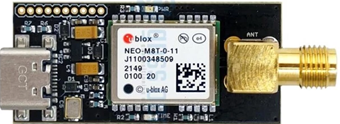
\includegraphics[width=6.1cm]{images/komponenty/GNSS_UBLOX.png}
\caption{GNSS přijímač Ublox NEO-M8T \cite{gnss_store}}
\end{figure}

\begin{figure}[H]
	\centering
	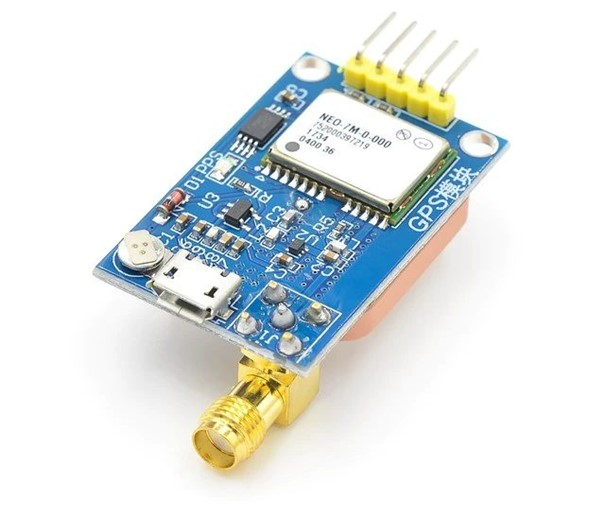
\includegraphics[width=6cm]{images/komponenty/UBLOX_NEO_7M.jpg}
	\caption{GNSS přijímač Ublox NEO 7M \cite{dratek_web}}
\end{figure}

\section{Čtečka Micro SD karet}
Protože Arduino samo o sobě nemá paměť pro ukládání dat, tak byla pro ukládání měřených dat využita Micro SD karta. Čtečka Micro SD karet umožňuje zapisovat měřená data na Micro SD kartu a popřípadě je z~ní i číst. Pro komunikaci s~čtečkou Micro SD karet je využíváno standardní SPI rozhraní \cite{arduino_navody}.

\begin{figure}[H]
	\centering
	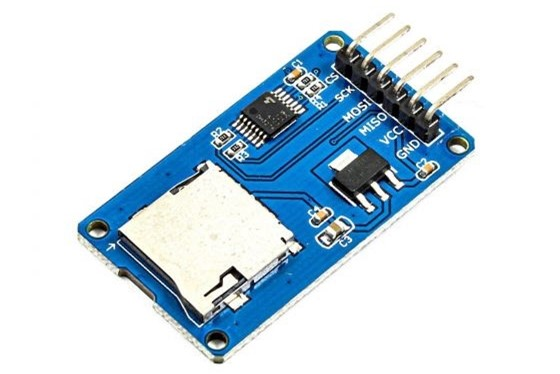
\includegraphics[width=6cm]{images/komponenty/ctecka_micro_sd.jpg}
	\caption{Čtečka Micro SD karet \cite{dratek_web}}
\end{figure}

\section{Tlačítko}
Tlačítko je jednoduchý komponent, sloužící pro detekci svého stisknutí. Stisknutí tlačítka slouží k~provedení záznamu času na Micro SD kartu. Místo samostatného tlačítka byl využit modul rotačního enkodéru, který umí detekovat své stisknutí a při pootočení osou poskytuje informaci o~směru rotace. Výhodou rotačního enkodéru oproti tlačítku je, že poskytuje další informace, které lze využít k~ovládání zařízení. Výhodou tohoto konkrétního modulu je to, že jej lze snadno upevnit ke krabičce s~výsledným zařízením.
\begin{figure}[H]
	\centering
	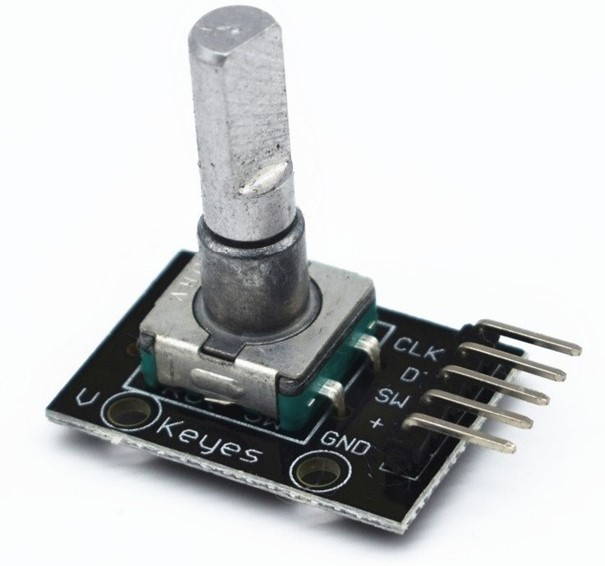
\includegraphics[width=4cm]{images/komponenty/rotacni_enkoder.jpg}
	\caption{Rotační enkodér \cite{dratek_web}}
\end{figure}

\section{OLED displej}
K~informování měřiče o~průběhu měření slouží mimo jiné displej. Na něj se zobrazuje informace o~stavu vložení Micro SD karty, o~stavu synchronizace času, aktuální čas a poslední uložený čas. Jako displej byl zvolen OLED displej především kvůli nízké ceně, dobré čitelnosti, nízké spotřebě energie a absenci potřeby dodatečného podsvícení, jelikož světélkují samotné pixely. Displej je monochromatický a jeho rozlišení je 128×64 bodů. K~řízení displeje je využívána komunikace pomocí I\(^2\)C sběrnice \cite{arduino_navody}.

\begin{figure}[H]
	\centering
	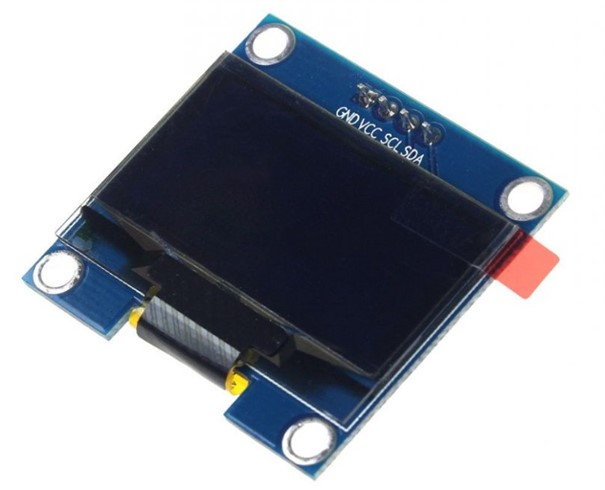
\includegraphics[width=5.4cm]{images/komponenty/displej.jpg}
	\caption{OLED displej \cite{dratek_web}}
\end{figure}

\section{Hlasový modul}
O~průběhu měření je měřič informován kromě displeje i pomocí reproduktoru, tak aby nemusel při měření sledovat displej. Měřiče o~průběhu měření informují slovní pokyny „Čas byl synchronizován“ a „Měření času bylo uloženo“, které byly vytvořeny pomocí převodu textu na mp3 soubor. Jelikož Arduino neumožňuje ukládat žádné soubory do své vnitřní paměti, tak jsou mp3 soubory se zvukovými informacemi nahrány na Micro SD kartu. Soubory jsou z~Micro SD karty čteny pomocí hlasového modulu a přehrávány pomocí reproduktoru, který je k~hlasovému modulu připojen. Hlasový modul s~Arduinem komunikuje prostřednictvím sériové komunikace \cite{arduino_navody}.

\begin{figure}[H]
	\centering
	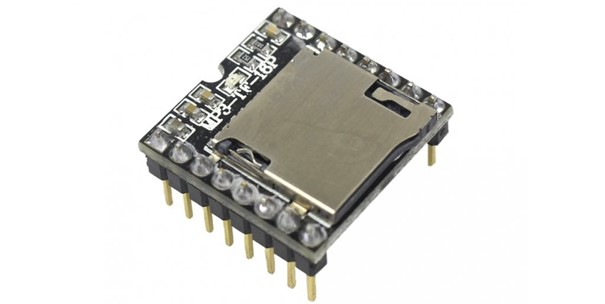
\includegraphics[width=7cm]{images/komponenty/DF_Player.jpg}
	\caption{Hlasový modul \cite{laskakit_web}}
\end{figure}

\begin{figure}[H]
	\centering
	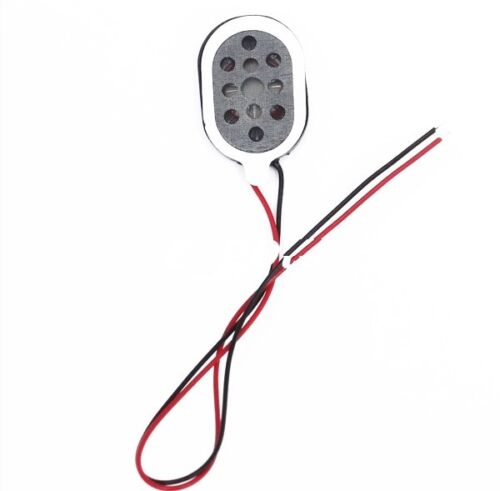
\includegraphics[width=4cm]{images/komponenty/reproduktor.jpg}
	\caption{Reproduktor \cite{arduino}}
\end{figure}

\section{RGB LED}
Kromě displeje a zvukového signálu je měřič informován o~průběhu měření také prostřednictvím elektroluminiscenční diody (\zk{LED}, z~anglického Light Emitting Diode). Jako \zkratka{LED} je využit modul RGB \zk{LED}, který se skládá ze tří samostatných \zk{LED} (červená, zelená, modrá). Tyto \zk{LED} mají společnou \text{katodu}, ale samostatné anody. K ovládání jasu jednotlivých barev slouží \zkratka{PWM}. Jednotlivé anody lze nezávisle na sobě připojit na piny s podporou \zk{PWM}, což umožňuje ovládat samostatně jednotlivé barvy. Další výhodou tohoto modulu je, že již má integrované ochranné rezistory. Během měření může \zk{LED} signalizovat různé stavy: Nejprve bliká červeně v~každý okamžik, kdy přijme signál DCF77 (v~ideálním případě je to jednou za sekundu). Ve chvíli, kdy je čas poprvé synchronizován se změní červené blikání na zelené, což informuje měřiče o~úspěšné synchronizaci času. Dále \zk{LED} bliká modře v~každý okamžik, kdy měřič provede měření \cite{arduino_navody}.
\begin{figure}[H]
	\centering
	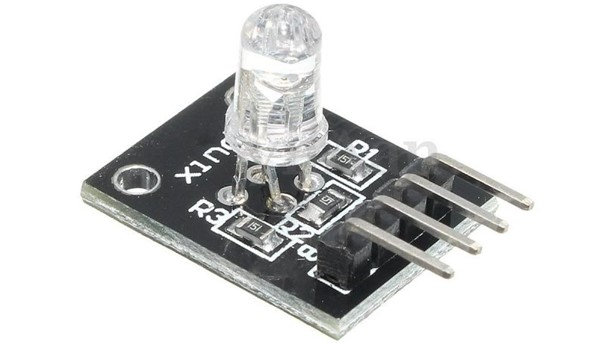
\includegraphics[width=6cm]{images/komponenty/RGB_LED.jpg}
	\caption{Modul s~RGB LED \cite{dratek_web}}
\end{figure}

\section{Převodník TTL na RS232}
Aby byl spolu s~časovými údaji uložen na Micro SD kartu vodorovný směr (a případně i zenitový úhel) měřený totální stanicí, je potřeba zajistit komunikaci Arduina s~totální stanicí. K~tomu lze využít sériovou komunikaci pomocí UART. Konkrétně byla využita totální stanice Leica TC1700. Ta využívá pro sériovou komunikaci standart RS-232 a lze k~ní tedy připojit sériový kabel RS-232 \cite{tps-dna}. Standart RS-232 využívá pro datové signály +3~V až +25~V jako logickou nulu a -3~V až -25~V jako logickou jedničku. Arduino UNO využívá protokol TTL, který považuje hodnoty okolo 0~V za logickou nulu a hodnoty v~okolí +5~V za logickou jedničku. Aby mohl být kabel RS-232 připojen i k~Arduinu, je potřeba využít převodník TTL na RS-232 \cite{sparkfun-tutorial}.

\begin{figure}[H]
	\centering
	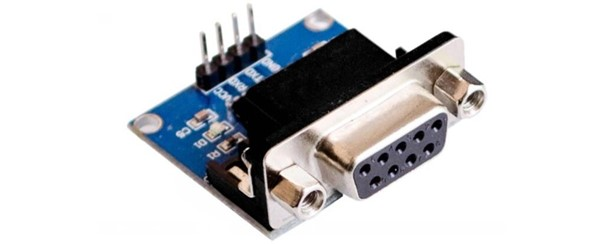
\includegraphics[width=8.5cm]{images/komponenty/prevodnik.jpg}
	\caption{Převodník TTL na RS232 \cite{laskakit_web}}
\end{figure}

\section{Bluetooth modul}
Pro export dat z~Micro SD karty, aniž by bylo potřeba ji vyjmout, lze využít \text{Bluetooth} modul. Konkrétně byl pro tento účel využit modul HC-05. Tento modul využívá sériovou komunikaci pomocí UART a podporuje Bluetooth ve verzi 2.0. Pomocí Bluetooth modulu lze přenášet binární data. Modul je připojen pomocí pinů GND, VCC, RX a TX. Kromě toho obsahuje piny STATE a EN, které slouží pro konfiguraci modulu. Pin EN na modulu HC-05 umožňuje přepnutí modulu do režimu „enabled“. V~tomto režimu lze pomocí AT příkazů nastavit jméno, heslo, popřípadě i baud rate a další parametry modulu \cite{arduino_navody}.

\begin{figure}[H]
	\centering
	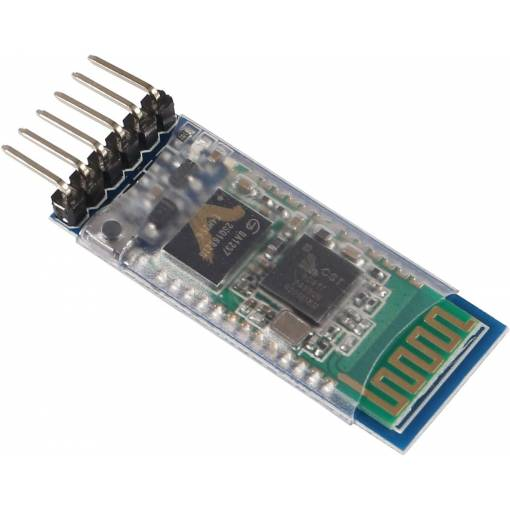
\includegraphics[width=4.6cm]{images/komponenty/BLUETOOTH-HC05.jpg}
	\caption{Bluetooth modul HC-05 \cite{dratek_web}}
\end{figure}

\section{Deska plošných spojů}
Během vývoje zařízení byly všechny komponenty spojovány pomocí kabelů. Nevýho\-dou propojení pomocí kabelů je velká prostorová náročnost a celková nepřehlednost. Z~toho důvodu bývá obvykle propojení různých komponentů realizováno pomocí desky plošných spojů. Pro snadné propojení všech využitých komponentů byla tedy vyhotovena \zkratka{DPS}.

\begin{figure}[H]
	\centering
	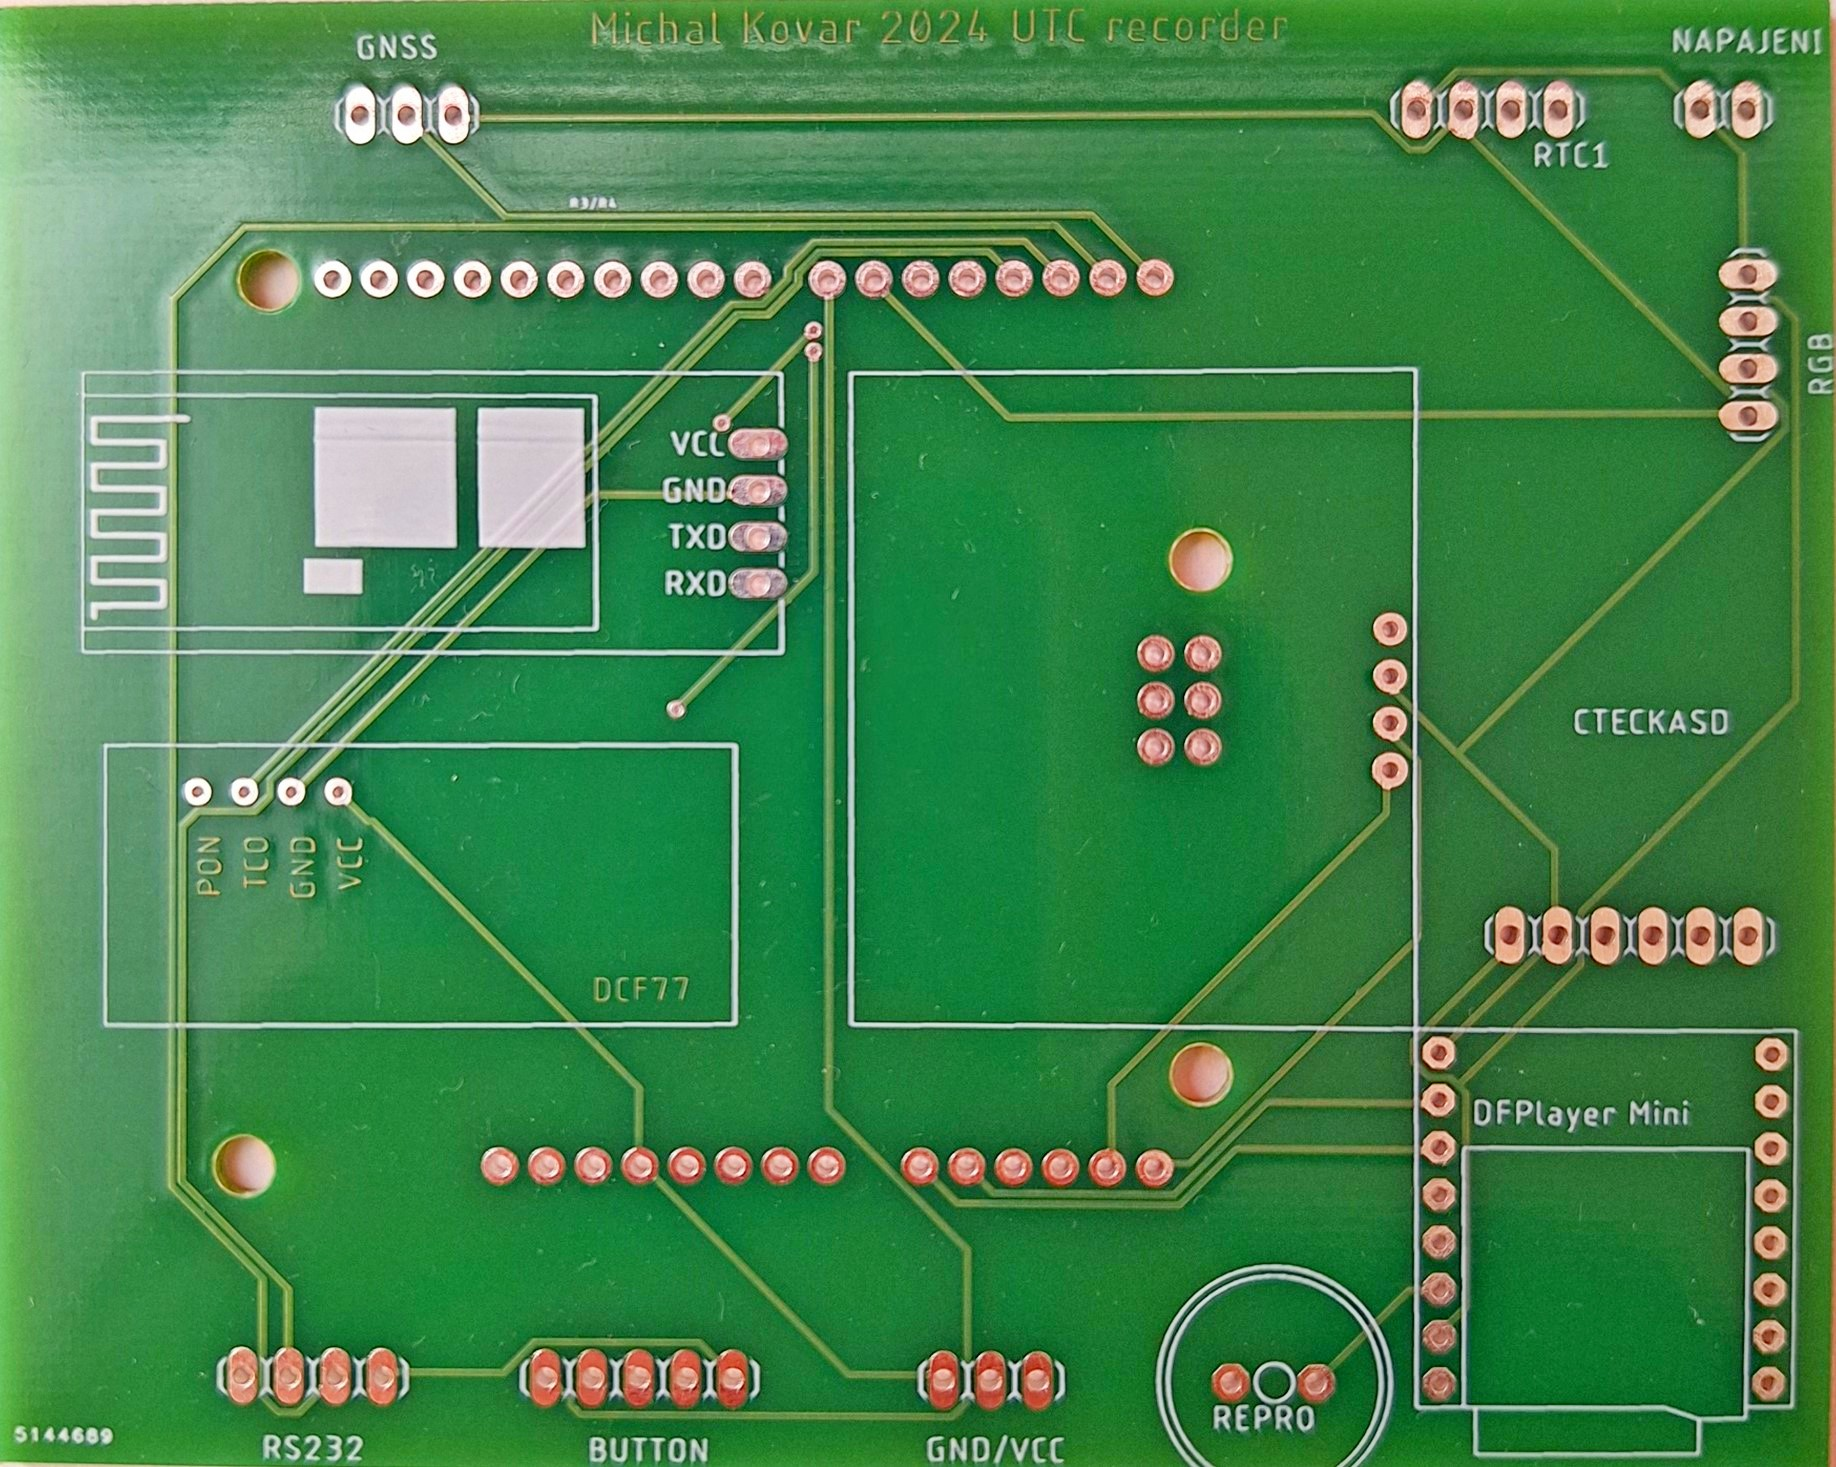
\includegraphics[width=5cm]{images/komponenty/dps_foto.jpg}
	\caption{Výsledná DPS}
\end{figure}

\section{Cena komponentů}
Ceny jednotlivých komponentů se mění v čase a mohou se lišit v závislosti na místě (obchodě), kde byly zakoupeny. Cena výsledného zařízení závisí na tom, zda byly použity všechny komponenty pro plnou funkcionalitu, nebo zda byly některé funkce vynechány.  Pokud se zařízení vyrábí s omezenou funkcionalitou, lze využít levnější Arduino UNO R3. Náklady na výsledné zařízení lze také snížit použitím „klonů“ místo originálního Arduina. Níže uvedená tabulka obsahuje komponenty potřebné pro zařízení s plnou funkcionalitou a uvádí ceny, za které byly tyto komponenty zakoupeny.

\begin{table}[H]
    \centering
    \caption{Cena použitých součástek}
    \begin{tabular}{|c|c|c|}
    \hline
    \textbf{Název} & \textbf{Cena} & \textbf{Odkaz na obchod}\\
    \hline\hline
    Arduino UNO R4 WiFi         & 768 Kč            & \href{https://www.laskakit.cz/arduino-uno-r4-wifi--original/}{laskakit.cz}  \\ \hline
    Přijímač DCF77              & 5,60 \euro/140 Kč  & \href{https://www.pollin.de/p/dcf-empfangsmodul-dcf1-810054}{pollin.de} \\ \hline
    Přijímač GNSS               & 339 Kč            & \href{https://dratek.cz/arduino/1733-gps-satelitni-urceni-polohy-neo-7m-modul.html?}{dratek.cz} \\ \hline
    Čtečka Micro SD karet       & 24 Kč             & \href{https://dratek.cz/arduino/993-ctecka-microsd-karet.html?}{dratek.cz} \\ \hline
    Tlačítko (rotační enkodér)   & 38 Kč             & \href{https://dratek.cz/arduino/837-rotacni-enkoder.html?}{dratek.cz} \\ \hline
    OLED displej                & 167 Kč            & \href{https://dratek.cz/arduino/3181-iic-i2c-oled-1-3-displej-128x64-bily.html?}{dratek.cz} \\ \hline
    Hlasový modul               & 66 Kč             & \href{https://dratek.cz/arduino/4857-hlasovy-modul-s-integrovanym-mp3-prehravacem-dfplayer.html?}{dratek.cz} \\ \hline
    Reproduktor                 & 19 Kč             & \href{https://dratek.cz/arduino/1175-reproduktor-1w-8ohm.html?}{dratek.cz} \\ \hline
    RGB LED                     & 15 Kč             & \href{https://dratek.cz/arduino/837-rotacni-enkoder.html}{dratek.cz} \\ \hline
    Bluetooth modul HC-05       & 117 Kč            & \href{https://dratek.cz/arduino/1005-bluetooth-modul-hc-05.html?}{dratek.cz} \\ \hline
    Deska plošných spojů        & 9,34 \$/216 Kč    & \href{https://www.allpcb.com/}{allpcb.com} \\ \hline
     \textbf{Celkem}            & 1909 Kč           & - \\ \hline
    \end{tabular}\\
\end{table}



\chapter{Vývoj zařízení - Konstrukce}
\label{5-vyvoj-zarizeni-konstrukce}
V~této kapitole bude vysvětleno zapojení jednotlivých komponentů, které byly pop\-sány v~předchozí kapitole. Dále bude popsán návrh desky plošných spojů (\zk{DPS}), jenž byl vyhotoven v~softwaru Autodesk EAGLE. Bude vysvětleno, jak byla \zk{DPS} osazena jednotlivými komponenty. Nakonec bude popsáno, jak byl vytvořen prototyp výsledného zařízení.

\section{Schéma zapojení}
Arduino Uno disponuje různými typy pinů, které lze využít k~různým účelům. Při zapojování jednotlivých komponentů je důležité zohlednit specifickou funkcionalitu jednotlivých pinů. Nelze totiž připojit součástky na libovolné piny, ale je nutné je zapojit na piny, které disponují potřebnou funkcionalitou. Jeden pin může mít více funkcí najednou. Piny Arduina mohou sloužit například jako digitální vstupy/výstupy, analogové vstupy, \zk{PWM} (analogové výstupy s~modulací šířky pulzu), RX a TX pro sériovou komunikaci, SDA a SCL pro I\(^2\)C komunikaci nebo jako MISO, MOSI, CLK, a CS pro SPI komunikaci \cite{arduino}.

\begin{figure}[H]
	\centering
	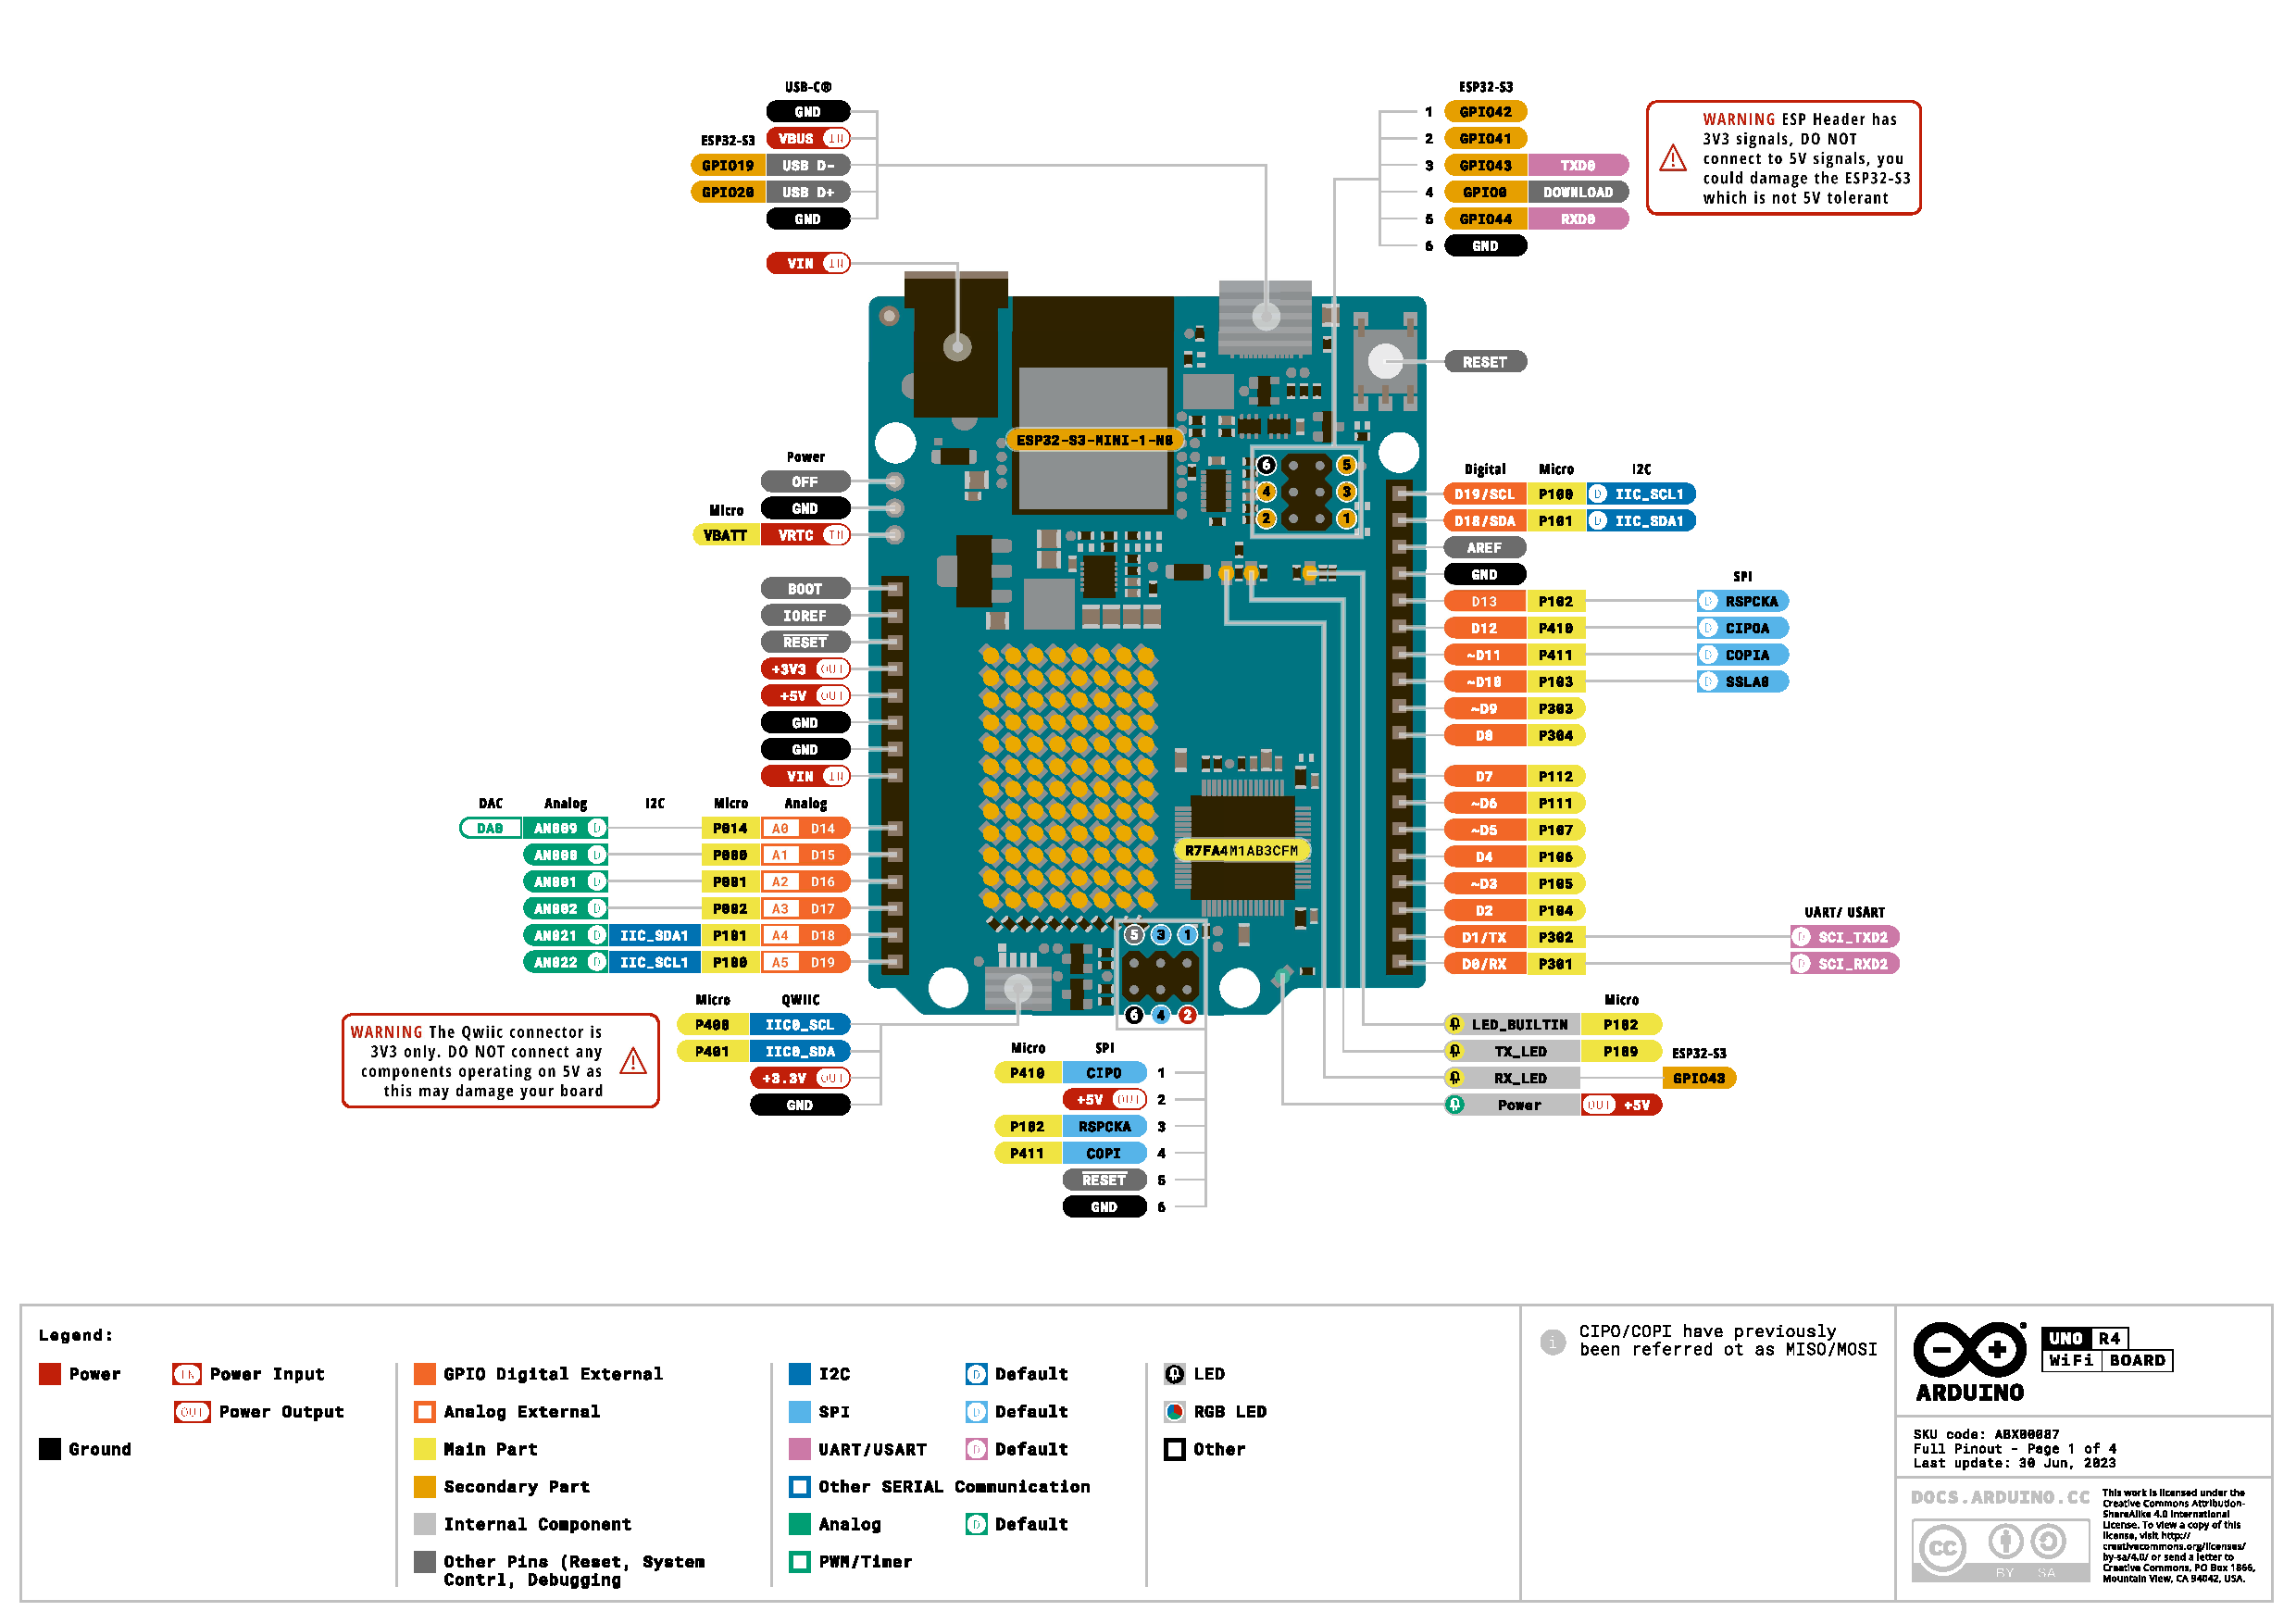
\includegraphics[width=14.9cm]{images/pinout_rotated.pdf}
	\caption{Výstupy pinů pro Arduino UNO R4 \cite{arduino}}
\end{figure}

Schéma zapojení bylo vyhotoveno v~softwaru Autodesk Eagle. nejprve bylo \text{vyhotoveno} schéma zapojení pro Arduino UNO R3 podle toho, jak byly jednotlivé komponenty zapojeny v~rámci testování jejich funkčnosti. Toto schéma zapojení sloužilo jako podklad pro tvorbu desky plošných spojů (\zk{DPS}). Arduino UNO R3 však nedisponuje dostatečnou kapacitou paměti k~tomu, aby mohlo \text{obsluhovat} všechny plánované komponenty. Pro finální zařízení, které bude disponovat plnou funkcionalitou, bylo proto zvoleno Arduino UNO R4. Vzhledem k~tomu, že Arduino UNO R4 má lehce odlišné rozvržení pinů oproti verzi R3, bylo nutné vyhotovit nové schéma zapojení a podle něj i novou \zk{DPS}. Nové schéma zapojení se povedlo navrhnout tak, že nová \zk{DPS} je kompatibilní s~oběma verzemi Arduina UNO (R3 i R4).

\begin{figure}[H]
	\centering
	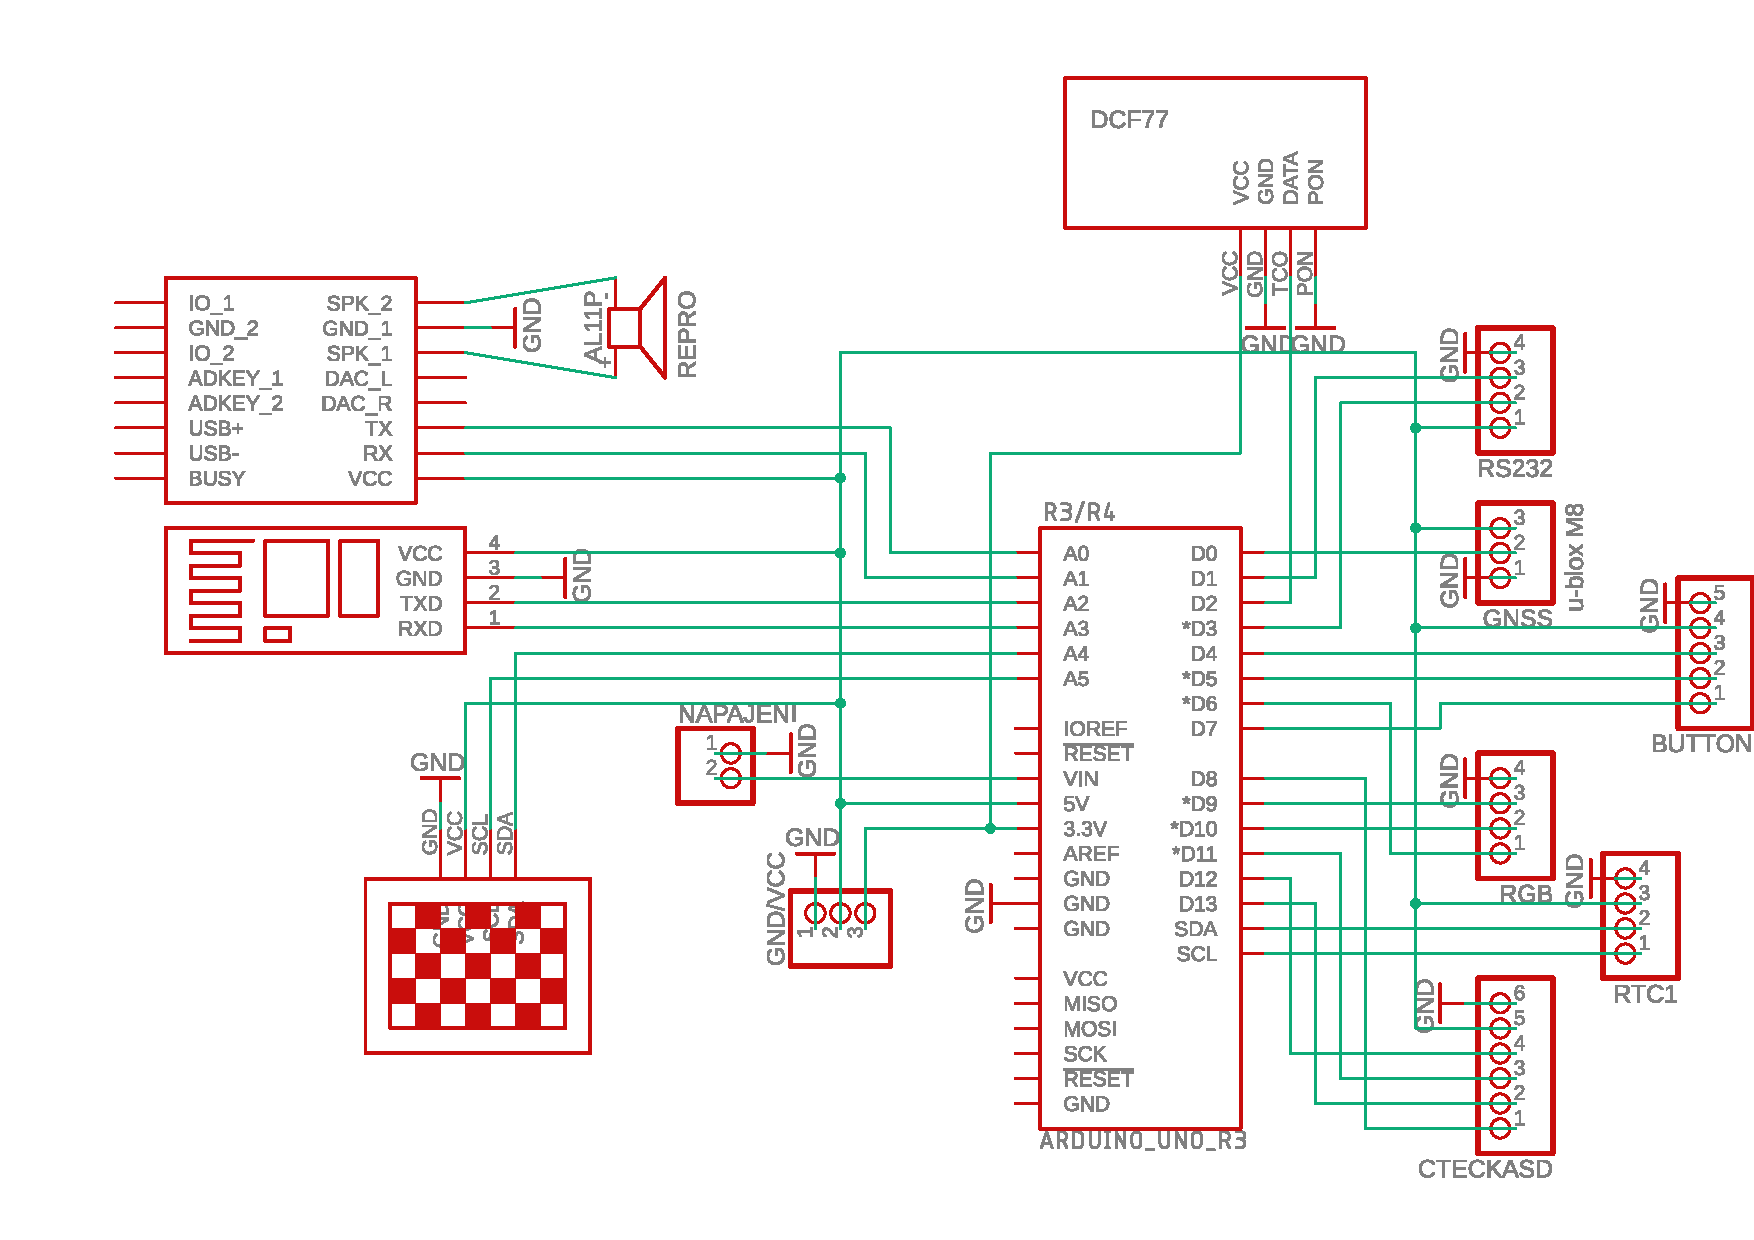
\includegraphics[width=14.1cm]{images/schema_zapojeni.pdf}
	\caption{Schéma zapojení komponentů pro Arduino Uno}
\end{figure}

\subsubsection*{Přijímač časového signálu DCF77}
Přijímač poskytuje digitální signál, který odpovídá dekódovaným bitům časového kódu.
Tento digitální signál je pak k~dispozici na výstupním pinu přijímače (obvykle označeném jako TCO nebo DATA), který je potřeba připojit k~digitálnímu vstupu Arduina.
\begin{itemize}
    \tiny
    \setlength{\itemsep}{0pt} 
    \item VCC $\rightarrow$ 3.3V
    \item GND $\rightarrow$ GND
    \item PON $\rightarrow$ GND
    \item TCO $\rightarrow$ D2
\end{itemize}

\subsubsection*{GNSS přijímač u-blox NEO}
Komunikace s~Arduinem probíhá pomocí sériové komunikace TTL přes rozhraní UART. Je nutné připojit přijímač k~pinům Arduina, které tuto komunikaci umožňují.
 \begin{itemize}
     \tiny
     \setlength{\itemsep}{0pt} 
     \item VCC $\rightarrow$ 5V 
     \item GND $\rightarrow$ GND
     \item TX  $\rightarrow$ D0
 \end{itemize}

    
\subsubsection*{Tlačítko (rotační enkodér)}
Rotační enkodér poskytuje digitální signály, které odpovídají jeho otáčení a stisknutí tlačítka. Tyto signály lze číst pomocí digitálních pinů Arduina, které mohou sloužit jako digitální vstupy.
\begin{itemize}    
    \tiny
    \setlength{\itemsep}{0pt} 
    \item VCC $\rightarrow$ GND
    \item GND $\rightarrow$ 5V
    \item CLK $\rightarrow$ D6
    \item DT  $\rightarrow$ D5
    \item SW  $\rightarrow$ D4
\end{itemize}

\subsubsection*{OLED displej}
OLED displej využívá i\(^2\)C komunikaci a je tedy potřeba jej připojit k~pinům, které ji podporují.
\begin{itemize}
    \tiny
    \setlength{\itemsep}{0pt} 
    \item VCC $\rightarrow$ 5V 
    \item GND $\rightarrow$ GND
    \item SDA $\rightarrow$ A4
    \item SCL $\rightarrow$ A5 
\end{itemize}

\subsubsection*{Hlasový modul}
Hlasový modul využívá sériovou komunikaci. Kvůli nedostatku sériových pinů na Arduinu UNO je použita knihovna SoftwareSerial, která umožňuje emulovat \text{sériovou} komunikaci pomocí některých pinů, které nejsou primárně určeny pro sériovou komu\-nikaci.
\begin{itemize}
    \tiny
    \setlength{\itemsep}{0pt} 
    \item VCC $\rightarrow$ 5V 
    \item GND $\rightarrow$ GND
    \item TX  $\rightarrow$ RX 
    \item RX  $\rightarrow$ TX
    \item SPK1 $\rightarrow$ reproduktor (+)
    \item SPK2 $\rightarrow$ reproduktor (-)
\end{itemize}

\subsubsection*{RGB LED}
Pro ovládání jasu světla jednotlivých barev, lze využít piny s~podporou pulzně šířkové modulace (\zk{PWM}), označené symboly „\(\sim \)“.
\begin{itemize}
    \tiny
    \setlength{\itemsep}{0pt} 
    \item R $\rightarrow$ \(\sim \)D9
    \item G $\rightarrow$ \(\sim \)D10
    \item B $\rightarrow$ \(\sim \)D11
    \item GND $\rightarrow$ GND
\end{itemize}

\subsubsection*{Bluetooth modul HC-05}
Bluetooth modul HC-05 využívá sériovou komunikaci, ale Arduino UNO nemá dosta\-tečný počet sériových pinů. Proto jsou využity piny, které umožňují softwarovou emulaci sériové komunikace obdobně jako u~hlasového modulu.
\begin{itemize}
    \tiny
    \setlength{\itemsep}{0pt} 
    \item VCC $\rightarrow$ 5V 
    \item GND $\rightarrow$ GND
    \item TX  $\rightarrow$ RX 
    \item RX  $\rightarrow$ TX 
\end{itemize}

\section{Návrh DPS}
Návrh \zk{DPS} byl vyhotoven v~softwaru Autodesk Eagle. Propojení mezi komponenty vycházeli z~již vytvořeného schématu zapojení. Bylo navrženo rozmístění komponentů na \zk{DPS}. Pomocí funkce „Autorouter“ byly automaticky vygenerovány optimální trasy spojů. Dále byl vyhotoven „gerberfile“. Ten slouží jako podklad pro výrobu. Výroba \zk{DPS} může být provedena amatérsky. K~tomu je potřeba speciální vybavení a určitá zručnost zhotovitele. Vzhledem k~náročnosti výroby kvalitní \zk{DPS} byla zvolena možnost nechat ji vyrobit profesionální firmou, na základě předloženého „gerberfile“. Tím je zajištěno, že je \zk{DPS} kvalitní a spolehlivá.

\begin{figure}[H]
	\centering
	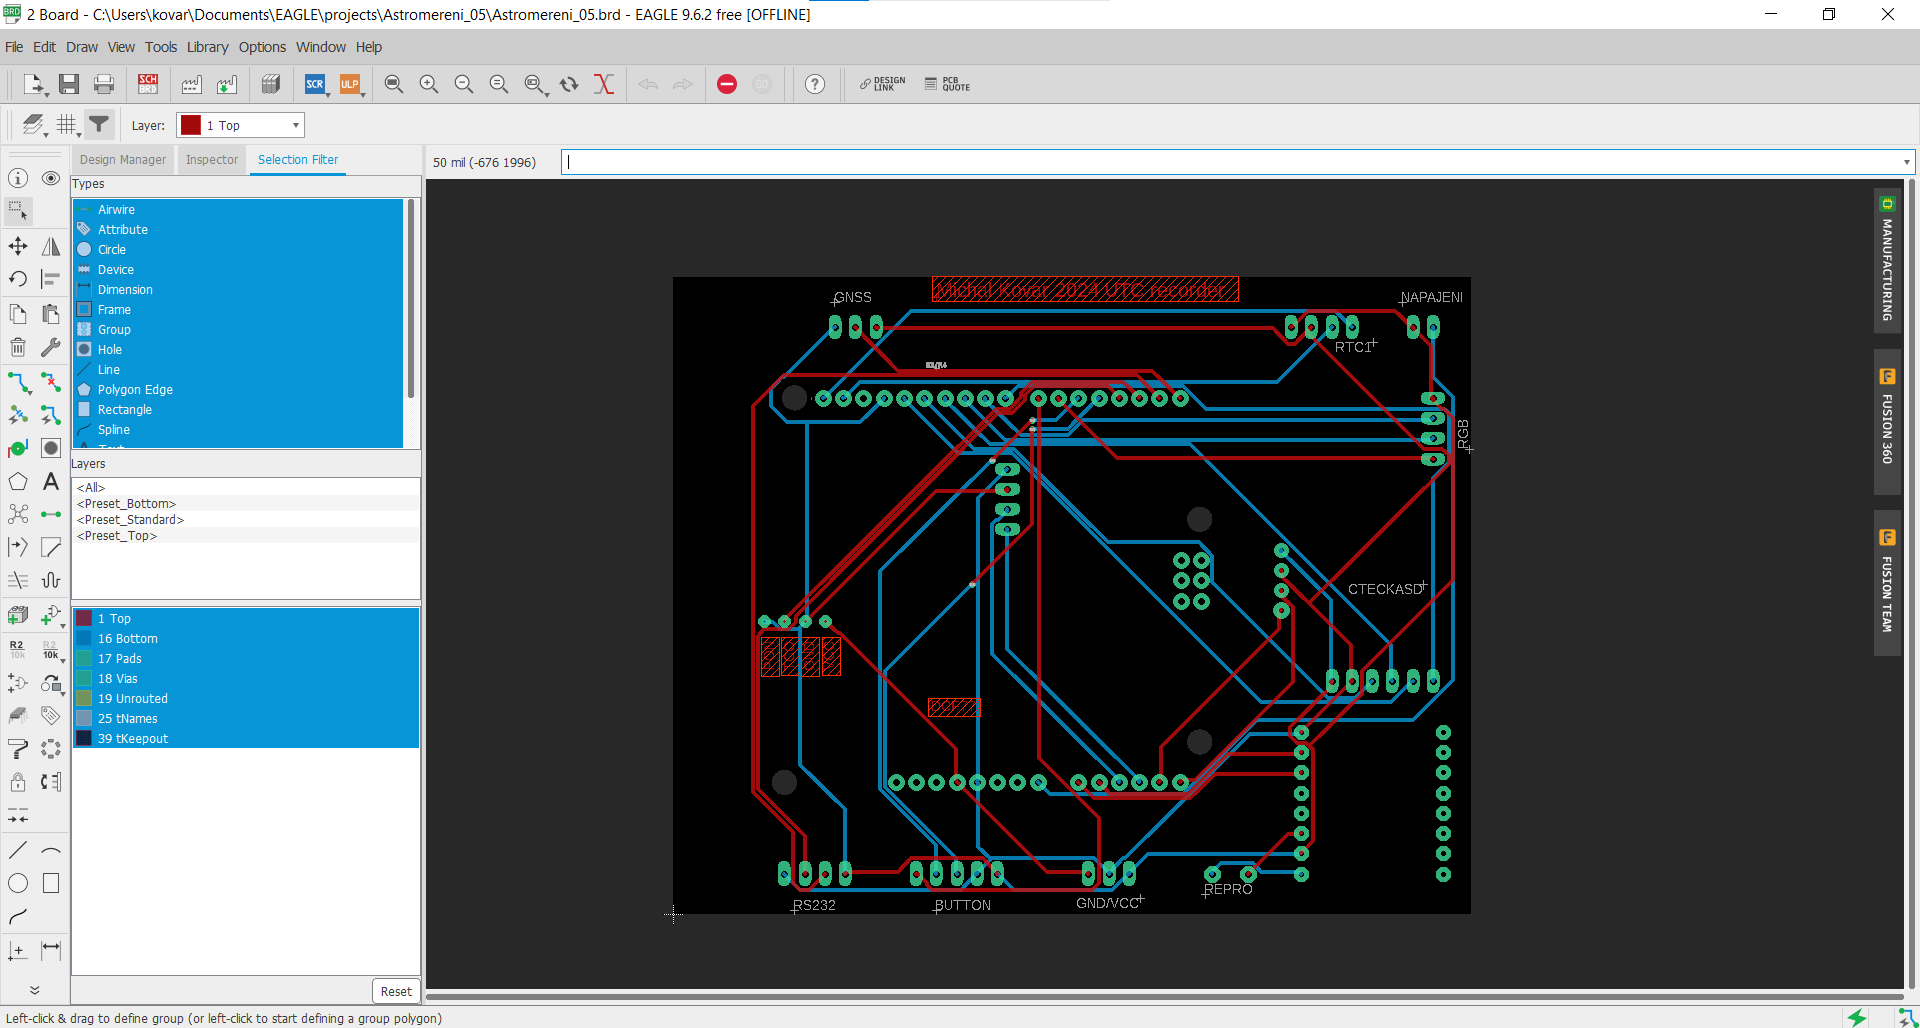
\includegraphics[width=15cm]{images/komponenty/EAGLE_NAVRH_DPS.png}
	\caption{Ukázka návrh DPS v~softwaru Autodesk Eagle}
\end{figure}

\section{Sestavení výsledného zařízení}
Deska plošných spojů byla navržena tak, aby společně s~komponenty k~ní připojenými bylo výsledné zařízení co nejkompaktnější. K~desce byly připájeny další komponenty anebo patice a hřebínky, do kterých budou komponenty zapojeny, aby bylo možné některé komponenty v~případě potřeby odpojit nebo vyměnit. Některé součástky, jako tlačítka a displej byly připojeny k~desce pomocí kabelů. To umožňuje snadné umístění těchto součástek na vnější část krabičky. Kabely lze snadno odpojit pro případ, že by bylo zařízení potřeba rozebrat například z~důvodu výměny nějakého komponentu. Napájení zařízení je řešeno pomocí 9~V~baterie, která je propojená s~piny VIN a GND Arduina.

\begin{figure}[H]
	\centering
	\includegraphics[width=6.8cm]{images/komponenty/Osazená_DPS.jpg}
	\caption{Ukázka osazené DPS pro prototyp zařízení}
\end{figure}

Nakonec byly všechny komponenty integrovány do krabičky, která slouží jako tělo zařízení (astrochronografu). Tělo prototypu zařízení založeného na Arduinu UNO R3 bylo provizorně vytvořeno ze svačinové krabičky, která svými rozměry poměrně dobře vyhovuje potřebám zařízení. Svačinová krabička byla jako tělo zařízení využita z~důvodu toho, že je snadno dostupná a není potřeba ji speciálně vyrábět, zároveň je její výhodou vodotěsnost a průhlednost. V~budoucnu je v~plánu vytvořit vlastní tělo zařízení, které bude kompaktnější a bude přesně vyhovovat účelům zařízení. Do krabičky byly vyvrtány a vyřezány díry pro displej, konektory a tlačítka, které jsou utěsněny silikonem, aby byla zachována vodotěsnost celého zařízení.

\begin{figure}[H]
	\centering
	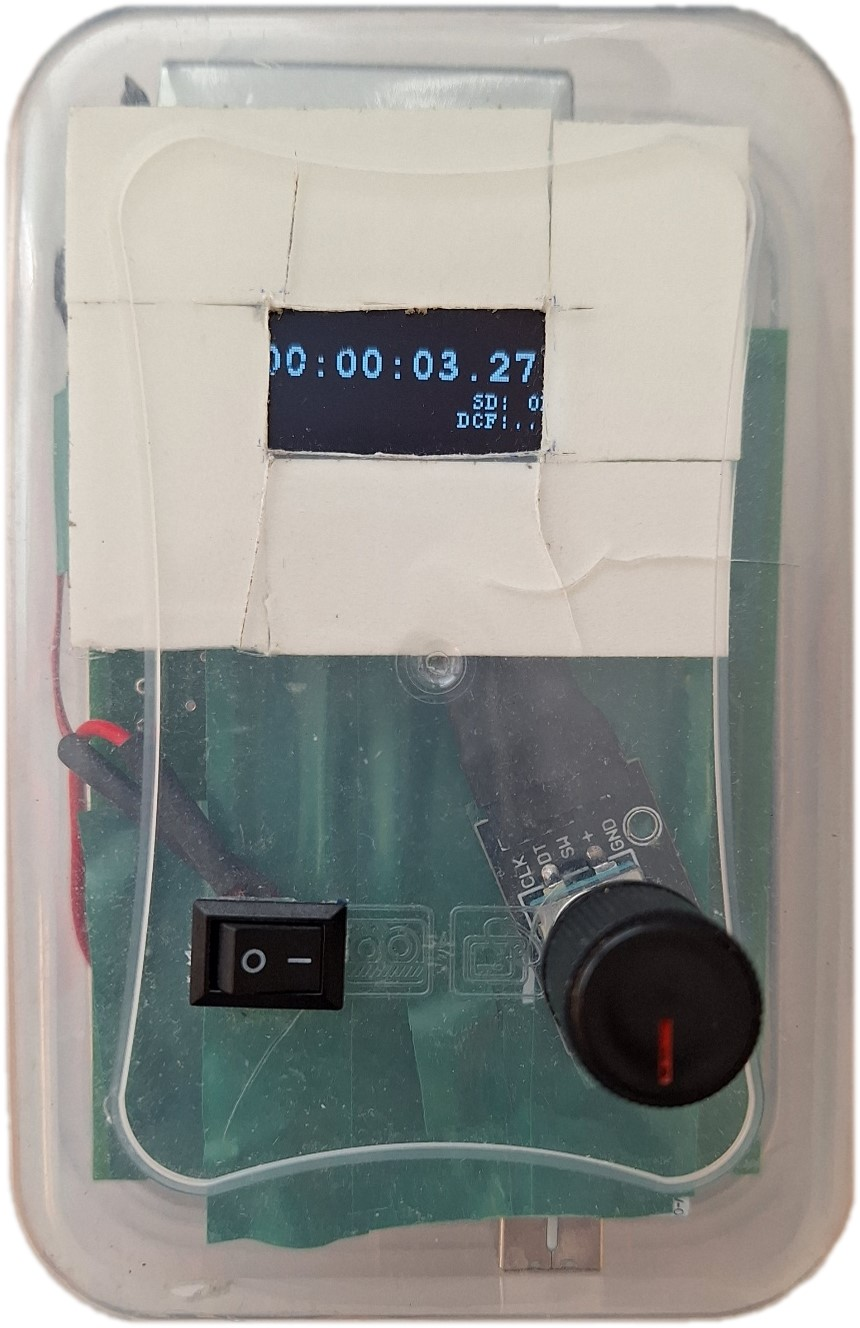
\includegraphics[width=10cm]{images/komponenty/prototyp2.jpg}
	\caption{Prototyp zařízení}
\end{figure}
\chapter{Vývoj zařízení - Řídící software}
\label{5-vyvoj-zarizeni-ridici-software}
%V této kapitole bude popsána tvorba řídícího programu pro Arduino.

\section{Programovací jazyk}

Nejběžněji bývá pro tvorbu řídícího programu pro Arduino využívána varianta jazyka C++, která využívá struktury převzaté z~jazyka Wiring. Alternativně lze použít jazyky jako MicroPython, JavaScript a další. Ve Wiringu se namísto typické funkce \texttt{main} pro C++ používají funkce \texttt{setup} pro prvotní inicializaci při spuštění programu a funkce \texttt{loop} pro nekonečnou smyčku, která program nepřetržitě vykonává \cite{arduino}.

\section{Vývojové prostředí}
Pro tvorbu a nahrání řídicího programu do mikrokontroléru se využívá \zkratka{IDE}. Mikrokontroléry, na rozdíl od jednodeskových mikropočítačů, nejsou vybaveny operačním systémem. Nelze tedy tvořit kód přímo na mikro\-kontroléru, je potřeba jej vytvořit na počítači, zkompilovat a následně nahrát jako binární soubor do mikro\-kontroléru. Pro tvorbu řídicího programu bylo konkrétně využito Arduino \zk{IDE}. To nabízí kromě možnosti psaní, kompilování a nahrávání kódu i správu knihoven a čtení dat z~Arduina pro ladění kódu. Kromě vývojového prostředí Arduino \zk{IDE} bylo využíváno prostředí VS Code od společnosti Microsoft, které umožňuje verzování pomocí Gitu a sdílení kódu na platformě GitHub.

\begin{figure}[H]
	\centering
	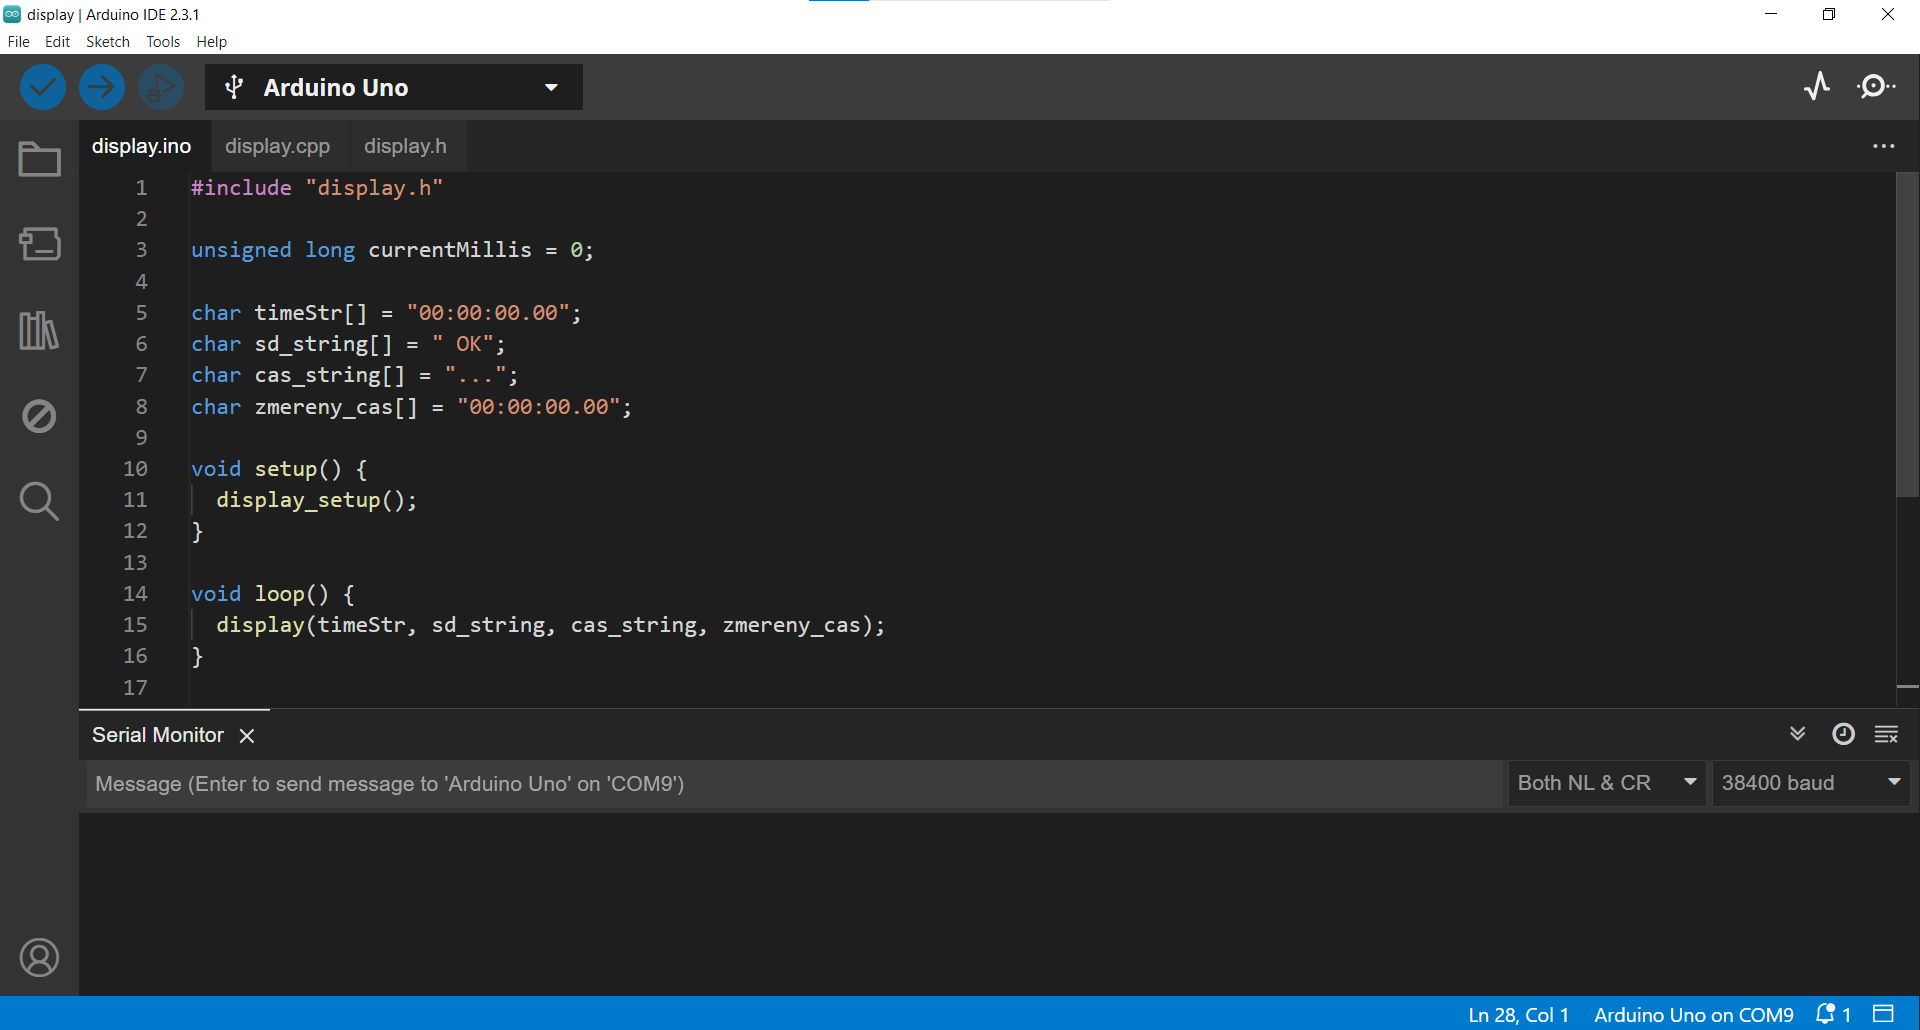
\includegraphics[width=14.5cm]{images/komponenty/Arduino_IDE.png}
	\caption{Arduino IDE}
\end{figure}

\section{Použité knihovny}
Pro práci s~některými komponenty byly využity již existující knihovny, které usnadňují využití jejich funkcionality. Knihovna \href{https://www.arduino.cc/en/Reference/SoftwareSerial}{\texttt{SoftwareSerial.h}} byla využita pro emulaci pinů sloužících pro sériovou komunikaci, protože Arduino UNO obsahuje pouze jeden TX a jeden RX pin, určený pro sériovou komunikaci. Pro práci s~údaji o~čase byla využita knihovna \href{https://www.pjrc.com/teensy/td_libs_Time.html}{\texttt{TimeLib.h}}. Pro synchronizaci času prostřednictvím signálu z~DCF77 přijímače byla využita knihovna \href{https://github.com/thijse/Arduino-DCF77}{\texttt{DCF77.h}}. Tato knihovna obsahuje funkce pro dekódování signálu DCF77. Pro přístup k~NTP serveru byly využity knihovny \href{https://github.com/esp8266/Arduino/tree/master/libraries/ESP8266WiFi}{\texttt{WiFiS3.h}} a \href{https://www.arduino.cc/en/Reference/WiFi}{\texttt{WiFiUdp.h}}. Ty slouží pro připojení k~WiFi a přijímaní a odesílání paketů, které využívá NTP server. Pro práci s~Micro SD kartou byla využita knihovna \href{https://www.arduino.cc/en/Reference/SD}{\texttt{SD.h}}. Tato knihovna obsahuje funkce pro zapisování dat na Micro SD kartu a čtení dat z~ní. Pro práci s~OLED displejem byla nejprve využívána knihovna \href{https://github.com/olikraus/u8glib}{\texttt{U8glib.h}}, která ale není kompatibilní s~mikrokontroléry Renesas, a tak byla využita knihovna \href{https://github.com/olikraus/u8g2}{\texttt{U8g2lib.h}}. Pro práci s~hlasovým modulem byla využita knihovna \href{https://github.com/DFRobot/DFRobotDFPlayerMini}{\texttt{DFRobotDFPlayerMini.h}}.

\section{Členění kódu}
Řídící program byl rozdělen z~důvodu přehlednosti na hlavní program \texttt{(*.ino)}, který sdružuje další části kódu ve formě hlavičkových (\texttt{*.h}) a implementačních souborů (\texttt{*.cpp}). Během tvorby řídícího programu byly využity již existující kniho\-vny a při tvorbě kódu bylo vycházeno ze vzorových kódů, které k~nim byly přiložené v~dokumentaci. Nicméně některé části kódu byly vytvořeny zcela nově. \text{Například} bylo potřeba zajistit, aby stisknutí tlačítka bylo považováno za stisknutí pouze v~prvním průchodu funkcí \texttt{loop}, a v~dalších průchodech již nebylo tlačítko považováno za stisknuté tak, aby bylo provedeno při každém stisku jen jedno měření a měření bylo přehledné a jednoznačné. Kód pro příjem dat z~GNSS přijímače byl vytvořen také kompletně od začátku. V~tomto kódu je načítána pomocí sériové komunikace NMEA zpráva. Ta je parsována a je z~ní zjišťováno, zda byla určena poloha přijímače. Pokud je určena poloha přijímače lze považovat čas za aktuální. V~tom případě je text s~časem převeden na číselné hodnoty a s~těmi je dále praco\-váno. Dalším pří\-kladem je funkce setiny. Jelikož všechny použité přijímače poskytují data po celých sekundách, tak byla vytvořena funkce setiny, která je spuštěna vždy na začátku celé sekundy a rozděluje ji na setiny sekund. Při každé nové sekundě jsou setiny sekund vynulovány. Od začátku byla také vyhotovena část kódu pro komunikaci s~totální stanicí a další části kódu.

\vspace{1cm}

\begin{figure}[H]
\hspace{-1cm}
\begin{tikzpicture}[
    startstop/.style={rectangle, rounded corners, minimum width=2cm, minimum height=0.5cm,text centered, draw=black, fill=red!30},
    io/.style={trapezium, trapezium left angle=70, trapezium right angle=110, minimum width=2cm, minimum height=0.5cm, text centered, draw=black, fill=blue!30},
    process/.style={rectangle, minimum width=2cm, minimum height=0.5cm, text centered, draw=black, fill=orange!30},
    decision/.style={diamond, minimum width=2cm, minimum height=0.5cm, text centered, draw=black, fill=green!30},
    arrow/.style={thick,->,>=stealth},
]

\node (init) [startstop] {Inicializace zařízení};
\node (sdCheck) [process, below of=init, yshift=-0.25cm] {Kontrola připojení micro SD karty};
\node (timeAttempt) [process, below of=sdCheck, yshift=-0.25cm] {Pokus o~aktualizaci času};
\node (display) [process, below of=timeAttempt, yshift=-0.25cm] {Zobrazení aktuálního stavu na displeji};
\node (buttonCheck) [decision, below of=display, yshift=-2cm, align=center] {Kontrola\\stisknutí\\tlačítka};
\node (saveTime) [process, right of=buttonCheck, xshift=5.5cm] {Uložení aktuálního času};
\node (tsRequest) [process, below of=saveTime, yshift=-0.25cm] {Odeslání požadavku TS};
\node (saveTsData) [process, below of=tsRequest, yshift=-0.25cm] {Uložení dat z~TS};
\node (info) [process, below of=saveTsData, yshift=-0.25cm] {Signalizace};
\node (btCheck) [decision, below of=buttonCheck, yshift=-3.75cm, align=center] 
{Kontrola\\ požadavku\\ Bluetooth};

\node (uzel) [startstop, left of=btCheck, xshift=-5cm, align=center, fill=white, draw=white] {};

\node (openFile) [process, below of=btCheck, yshift=-2.1cm] {Otevření souboru s~měřenými daty};
\node (sendData) [process, below of=openFile, yshift=-0.25cm] {Odeslání dat přes Bluetooth};

\draw [arrow] (init) -- (sdCheck);
\draw [arrow] (sdCheck) -- (timeAttempt);
\draw [arrow] (timeAttempt) -- (display);
\draw [arrow] (display) -- (buttonCheck);
\draw [arrow] (buttonCheck.east) -- ++(1,0) |- node[yshift=0.2cm] {ano} (saveTime.west);
\draw [arrow] (saveTime) -- (tsRequest);
\draw [arrow] (tsRequest) -- (saveTsData);
\draw [arrow] (saveTsData) -- (info);
\draw [arrow] (info) |- (btCheck);

\draw [arrow] (btCheck.west) -- ++(0,0) |- node[yshift=0.2cm,xshift=-2cm] {ne} (uzel.center);

\draw [arrow] (buttonCheck) -- node[anchor=east] {ne} (btCheck);
\draw [arrow] (btCheck) -- node[xshift=0.5cm] {ano} (openFile);
\draw [arrow] (openFile) -- (sendData);
\draw [arrow] (sendData) |- ++(0,-1) -- ++(-6,0) |- (sdCheck);

\end{tikzpicture}
\caption{Zjednodušené schéma řídícího programu}
\end{figure}




% https://bastlirna.hwkitchen.cz/zakladni-struktury-jazyka-wiring/

% https://www.arduino.cc/reference/en/
\chapter{Testování}
\label{6-testovani}

\section{Testování během vývoje}
Funkčnost jednotlivých komponentů a byla testována v~průběhu vývoje řídicího programu. Nejprve byla testována funkčnost každého komponentu samostatně. Poté byly komponenty postupně začleňovány do celkového zařízení a byla testována jejich vzájemná spolupráce a funkčnost jako celek.

\section{Testování výsledného zařízení}
Po dokončení prototypu zařízení byla ověřena jeho funkčnost. Protože prototyp je založen na Arduinu UNO R3, má pouze omezenou funkcionalitu. Prototyp umí synchronizovat svůj vnitřní čas buď pomocí DCF77 nebo GNSS přijímače. Tento čas umí po stisknutí tlačítka ukládat na Micro SD kartu. Dále umí informovat měřiče o~průběhu měření prostřednictvím displeje, zvuku a diody. Všechny tyto zmíněné funkce byly otestovány a jsou plně funkční.

\section{Testování DCF77}
U~přijímače signálu DCF77 bylo testováno, jak rychle je schopné výsledné zařízení synchronizovat svůj vnitřní čas a jak často bývá čas synchronizován po první synchronizaci.

\subsubsection{Prvotní synchronizace}
Bylo zjištěno, že prvotní synchronizace bývá za vhodných podmínek provedena mezi druhou až třetí minutou od spuštění. 

\subsubsection{Průběžná synchronizace}
Jak často zařízení synchronizuje svůj vnitřní čas, bylo testováno tím, že bylo \text{zařízení} spuštěno po dobu jednoho dne u~okna orientovaného na západ. Na Micro SD kartě se vytváří soubor \texttt{TEST.TXT}, který obsahuje informace o~tom, kdy došlo k~\text{aktualizaci} času pomocí DCF77. Tato data byla následně zpracována v~softwaru R, kde byl vykreslen histogram znázorňující sloupce pro jednotlivé hodiny, přičemž velikost sloupce značí, kolik synchronizací bylo během této hodiny provedeno.

\begin{figure}[H]
	\centering
	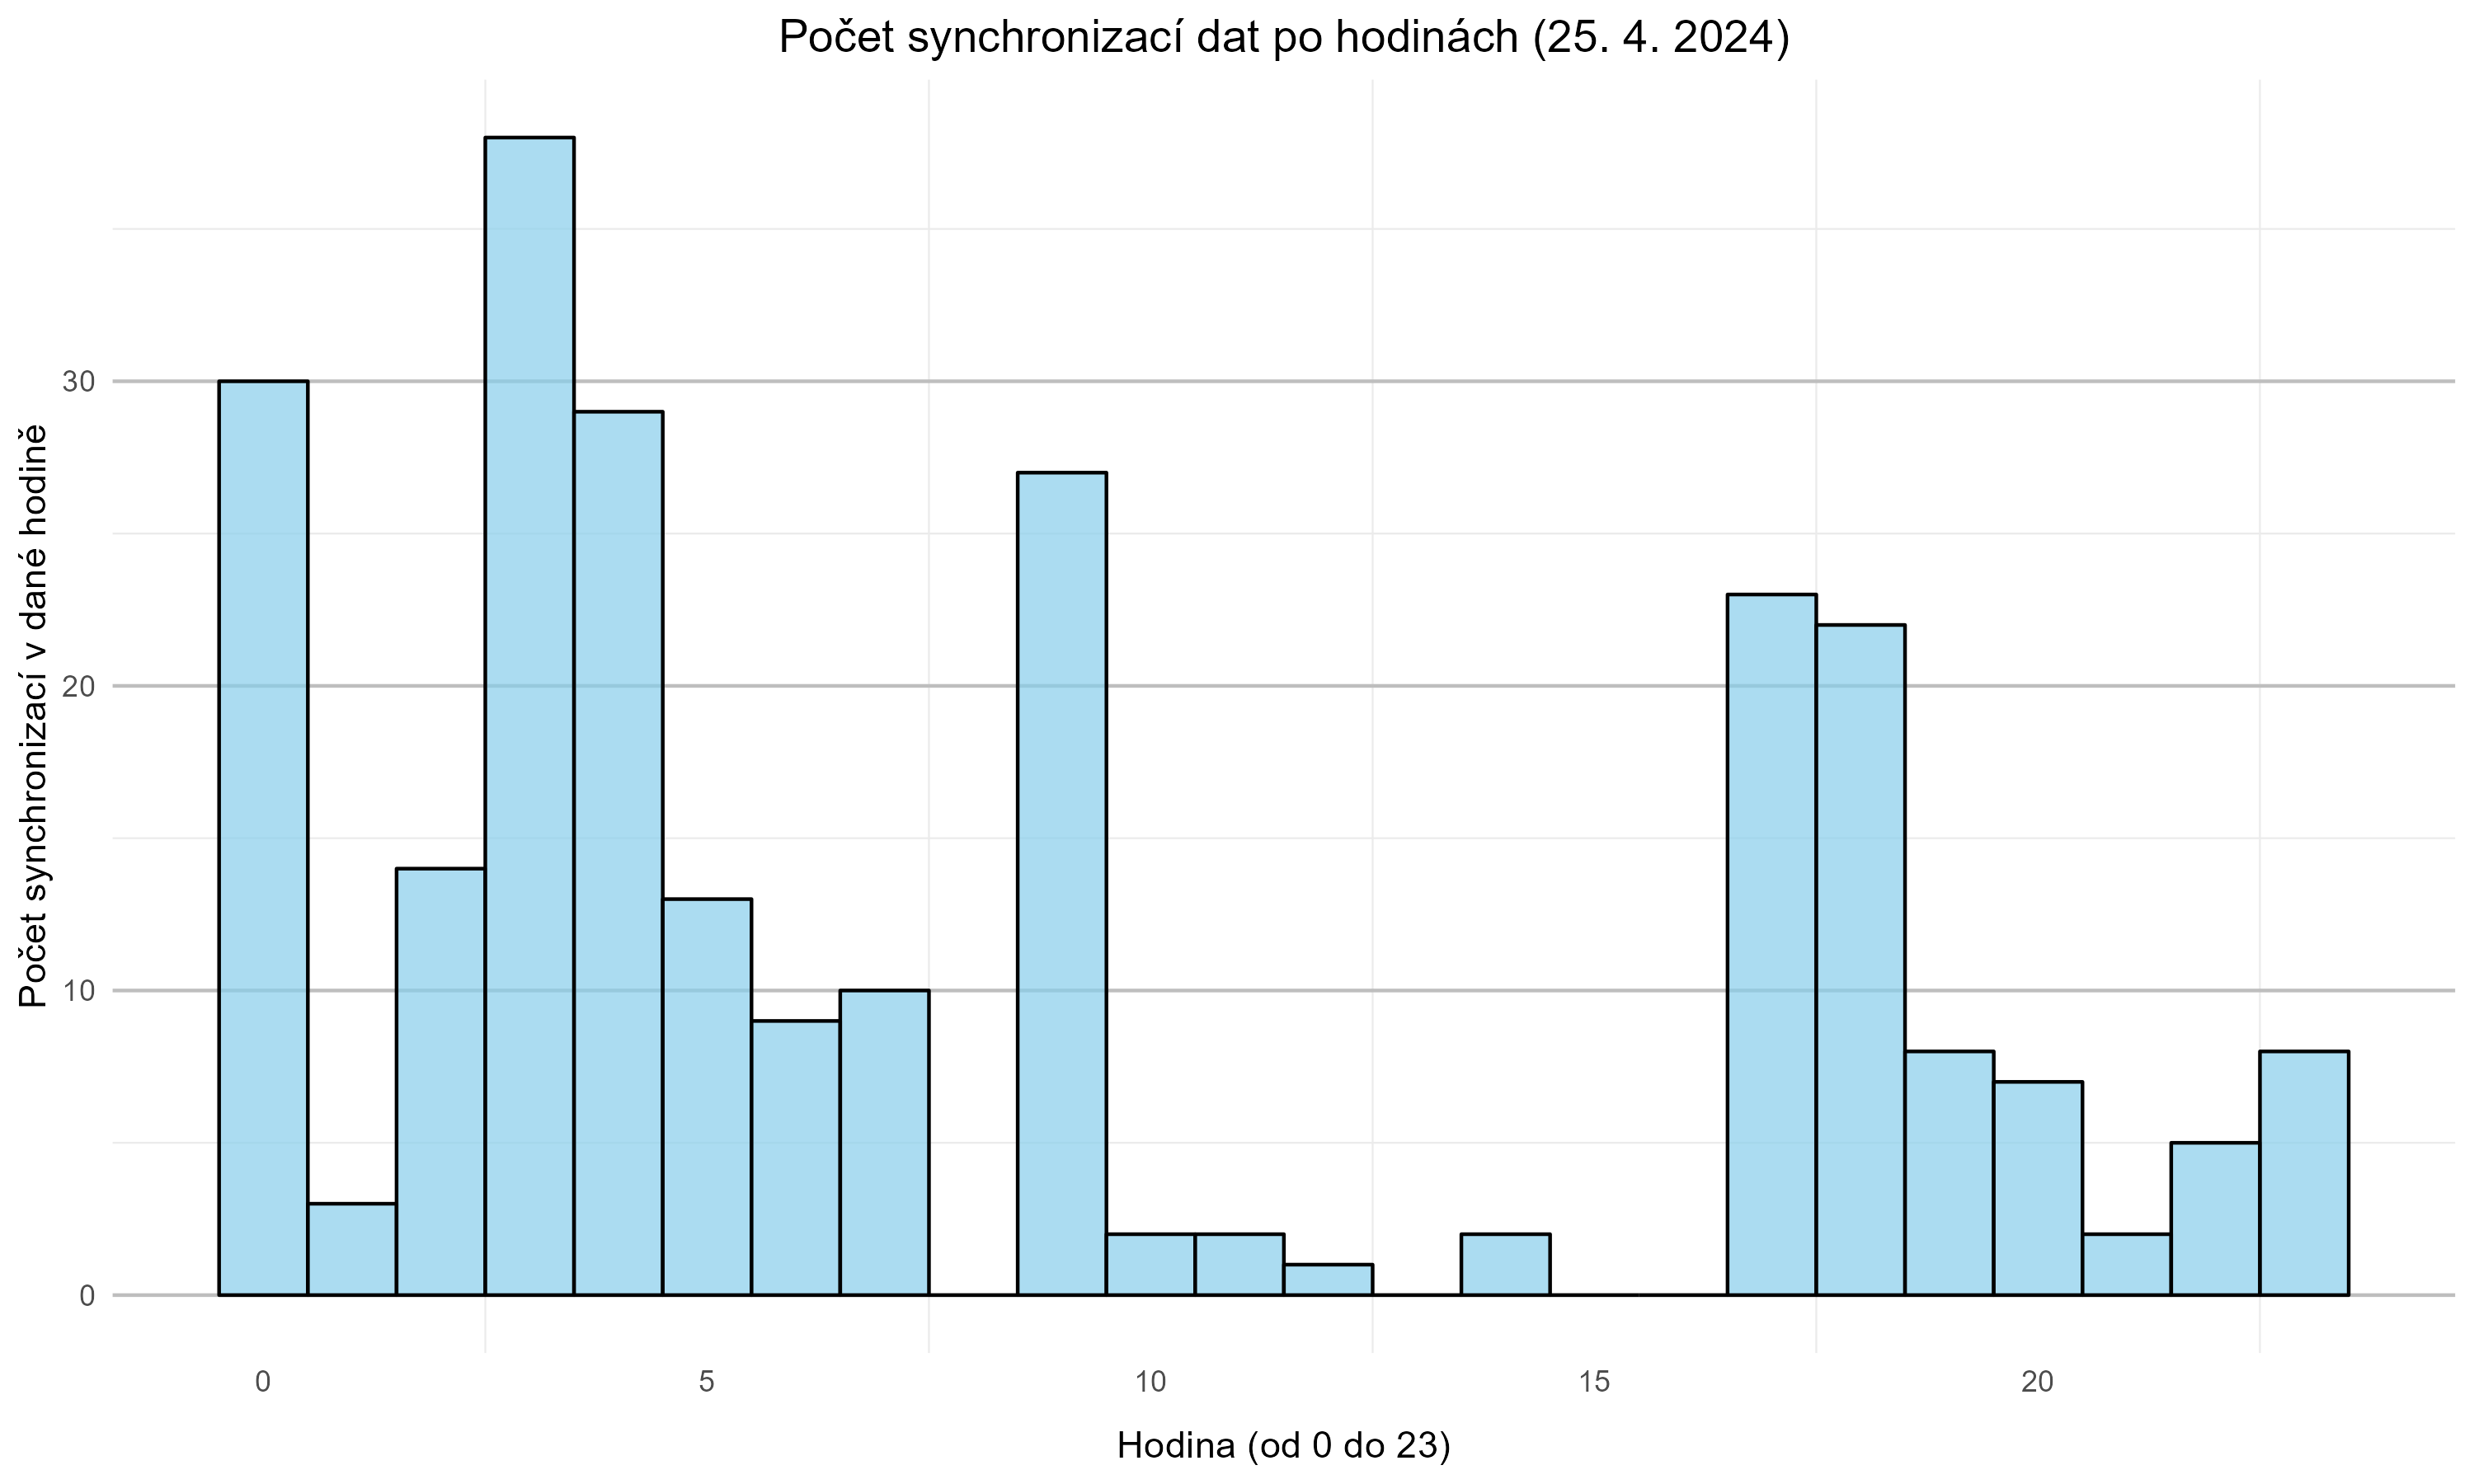
\includegraphics[width=12cm]{images/synchro_histogram.png}
	\caption{Histogram počtu synchronizací}
\end{figure}

\section{Testování GNSS modulu}

\subsubsection{Prvotní synchronizace}
Bylo zjištěno, že prvotní synchronizace bývá za vhodných podmínek (v~exteriéru nebo u~okna) provedena během několika sekund.

\subsubsection{Průběžná synchronizace}
Po prvotní synchronizaci získává modul čas nepřetržitě, pokud nedojde k~přerušení příjmu signálu (stínění antény).

\section{Testování NTP serveru}
Čas z~\zk{NTP} serveru bývá získán prakticky okamžitě a pokud nedojde k~přerušení internetového připojení získává zařízení čas nepřetržitě.

\section{Porovnání získaných časů}
Pro porovnání časů získaných z~NTP serveru, přijímače signálu DCF77 a GNSS přijímače byl vytvořen testovací kód pro Arduino UNO R4. Tento kód synchronizuje čas pomocí všech tří zmíněných metod a provádí záznam času každou minutu od spuštění Arduina.

\begin{table}[H]
    \centering
    \caption{Porovnání časů z~různých zdrojů}
    \begin{tabular}{|c|c|c|c|}
    \hline
    Arduino čas & NTP & DCF77 & GNSS \\
    \hline\hline
    00:04:00.00 & 10:27:12.52 & 10:27:12.55 & 10:27:12.68 \\ \hline
    00:05:00.00 & 10:28:12.50 & 10:28:12.55 & 10:28:12.65 \\ \hline
    00:06:00.00 & 10:29:12.49 & 10:29:12.55 & 10:29:12.64 \\ \hline
    00:07:00.00 & 10:30:12.49 & 10:30:12.54 & 10:30:12.69 \\ \hline
    00:08:00.00 & 10:31:12.48 & 10:31:12.54 & 10:31:12.62 \\ \hline
    \end{tabular}\\
\end{table}

Z~měřených dat je vidět, že získané časy se od sebe liší na úrovni setin až \text{desetin} sekundy. Tyto rozdíly mohou být způsobeny tím, že každý zdroj má lehce rozdílnou přesnost. \text{Nejvíce} se liší čas získaný pomocí GNSS přijímače, to může být způsobeno tím, že zpracování NMEA zprávy není dostatečně rychlé a dochází tedy ke zpoždění v~určení času. Pokud se chyba v~určení času pohybuje na úrovni pod jednu \text{desetinu} sekundy, lze očekávat, že chyba výsledného astronomického azimutu Slunce, způsobená určením času, bude mít velikost menší než 5\(^{cc}\).
\chapter{Závěr}
\label{7-zaver}

Cílem této práce bylo vytvořit zařízení pro příjem a záznam koordinovaného času určené pro účely astronomického měření (Astrochronograf). Toto zařízení má sloužit jako výuková pomůcka pro měření astronomických azimutů na Slunce v~rámci výuky teoretické geodézie.

Práce začala rešerší, během níž byly dohledány zdroje informací, týkající se témat spojených s~určováním času. Byly také dohledány cizí práce, které se zabývaly určováním času pro různé účely. Tyto zdroje poskytly informace o~tom, jakým vhodným způsobem při tvorbě zařízení lze postupovat.

V~teoretické části byly popsány jednotlivé typy časů a převody mezi nimi. Byl rozebrán vliv chyby při určování času na přesnost výsledných astronomických azi\-mutů. Nakonec byly zmíněny způsoby, jak lze synchronizovat čas zařízení.

V~praktické části byl navržen Astrochronograf. Byla vytvořena \zk{DPS} k~\text{propojení} všech využitých komponentů. Byl vytvořen řídící kód pro jednotlivé části zařízení. Dále byl vyhotoven prototyp zařízení, který je založen na Arduinu UNO R3. Z~dů\-vodu nedostatečné kapacity paměti Arduina UNO R3 má tento prototyp pouze omezenou funkcionalitu. Nicméně umožňuje synchronizaci času prostřednictvím \text{rádiového} \text{přijímače} DCF77 nebo prostřednictvím GNSS přijímače. Zařízení infor\-muje měřiče o~průběhu měření prostřednictvím displeje, \zk{LED} a zvukových pokynů tak, aby při měření nemusel měřič vizuálně sledovat zařízení.

Komponenty a pro ně vyhotovené řídící kódy, které nebyly do prototypu zahrnuty, byly samostatně testovány, jsou plně funkční a plánuje se jejich implementace do \text{zařízení}. Aby bylo možné tyto komponenty do zařízení implementovat, bude nutné vyměnit Arduino UNO R3 za Arduino UNO R4. Všechny komponenty a jejich řídící kódy byly testovány i na Arduinu UNO R4, a tak bude potřeba pouze fyzicky propojit komponenty. K~tomu bude sloužit nová deska plošných spojů, která je lehce jinak uspořádaná než \zk{DPS} použitá v~prototypu. Změna uspořádání komponentů na \zk{DPS} byla provedena z~důvodu, aby byla \zk{DPS} kompatibilní s~rozvržením pinů jak pro Arduino UNO R3, tak pro Arduino UNO R4. Tato \zk{DPS} bohužel dorazila až těsně před odevzdáním této práce, a tak je prozatím funkční pouze prototyp zařízení.

Tato práce je včetně zdrojových kódu veřejně dostupná na GitHubu, aby mohla sloužit jako zdroj informací pro lidi, kteří se budou v~budoucnu zabývat podobnými tématy.

% zařízení bylo vyztkoušeno a výstupem je zařízení které umí...

% Vysázení seznamu zkratek
\begin{seznamzkratek}{GNSS}
\novazkratka{API}{API}{Application Programming Interface}
\novazkratka{DPS}{DPS}{deska plošných spojů}
\novazkratka{GNSS}{GNSS}{globální navigační satelitní systémy}
\novazkratka{IDE}{IDE}{integrované vývojové prostředí} \(\) - z angl. Integrated Development Environment
\novazkratka{LED}{LED}{elektroluminiscenční dioda} \(\) - z angl. Light Emitting Diode
\novazkratka{NTP}{NTP}{Network Time Protokol}

\novazkratka{PWM}{PWM}{pulzně šířková modulace} \(\) - z angl. Pulse Width Modulation

\novazkratka{TAI}{TAI}{mezinárodní atomový čas} \(\) - z fr. Temps Atomique International
\novazkratka{UTC}{UTC}{univerzální koordinovaný čas}\(\) - z angl. Coordinated Universal Time / fr. Temps Universel Coordonné

%SI sistem international

%\novazkratka{VLBI}{VLBI}{interferometrie z velmi dlouhých základen} \(\) - z angl. Very-long-baseline interferometry
%\novazkratka{SEČ}{SEČ}{středoevropský čas}
%\novazkratka{SELČ}{SELČ}{středoevropský letní čas}
%\novazkratka{UART}{UART}{Universal asynchronous receiver-transmitter}

\end{seznamzkratek}

% Literatura
\nocite{*}
\def\refname{Literatura}
\bibliographystyle{mystyle}
\bibliography{literatura}


% Začátek příloh
\def\figurename{Figure}%
%\prilohy

% Vysázení seznamu příloh
\seznampriloh

% Vložení souboru s přílohami
% %%%%%%%%%%%%%%%%%%%%%%%%%%%%%%%%%%%%%%%%%%%%%%%%%%%%%%%%%%%%%%%%%%%%%%%%%%%%%%%%%%%
% %%                                    PŘÍLOHY                                    %%
% %%%%%%%%%%%%%%%%%%%%%%%%%%%%%%%%%%%%%%%%%%%%%%%%%%%%%%%%%%%%%%%%%%%%%%%%%%%%%%%%%%%

\appendix
% Příloha A: GitHub repozitář
\chapter*{A GitHub repozitář}
\addcontentsline{loa}{section}{A GitHub repozitář}
\href{https://github.com/kovarmi9/BachelorThesis-Astrochronograph}{\texttt{https://github.com/kovarmi9/BachelorThesis-Astrochronograph}}.
\begin{center}
\qrcode[height=4cm]{https://github.com/kovarmi9/BachelorThesis-Astrochronograph}
\end{center}
\textbf{Struktura repozitáře:}
\dirtree{%
.1 \href{https://github.com/kovarmi9/BachelorThesis-Astrochronograph}{BachelorThesis-Astrochronograph}.
.2 \href{https://github.com/kovarmi9/BachelorThesis-Astrochronograph/blob/main/README.md}{README.md}.\dottedline  stručná dokumentace.
.2 \href{https://github.com/kovarmi9/BachelorThesis-Astrochronograph/blob/main/src}{src}.
.3 \href{https://github.com/kovarmi9/BachelorThesis-Astrochronograph/tree/main/src/Arduino}{Arduino}.\dottedline kódy pro Arduino.
.4 \href{https://github.com/kovarmi9/BachelorThesis-Astrochronograph/tree/main/src/Arduino/Components}{Components}.\dottedline kódy pro jednotlivé komponenty.
.5 \href{https://github.com/kovarmi9/BachelorThesis-Astrochronograph/tree/main/src/Arduino/Components/BLE}{BLE}.
.5 \href{https://github.com/kovarmi9/BachelorThesis-Astrochronograph/tree/main/src/Arduino/Components/Bluetooth}{Bluetooth}.
.5 \href{https://github.com/kovarmi9/BachelorThesis-Astrochronograph/tree/main/src/Arduino/Components/DCF77_time}{DCF77\_time}.
.5 \href{https://github.com/kovarmi9/BachelorThesis-Astrochronograph/tree/main/src/Arduino/Components/Display}{Display}.
.5 \href{https://github.com/kovarmi9/BachelorThesis-Astrochronograph/tree/main/src/Arduino/Components/GNSS_time}{GNSS\_time}.
.5 \href{https://github.com/kovarmi9/BachelorThesis-Astrochronograph/tree/main/src/Arduino/Components/NTP}{NTP}.
.5 \href{https://github.com/kovarmi9/BachelorThesis-Astrochronograph/tree/main/src/Arduino/Components/RGB_LED}{RGB\_LED}.
.5 \href{https://github.com/kovarmi9/BachelorThesis-Astrochronograph/tree/main/src/Arduino/Components/Rotarry_encoder}{Rotarry\_encoder}.
.5 \href{https://github.com/kovarmi9/BachelorThesis-Astrochronograph/tree/main/src/Arduino/Components/RTC}{RTC}.
.5 \href{https://github.com/kovarmi9/BachelorThesis-Astrochronograph/tree/main/src/Arduino/Components/SD}{SD}.
.5 \href{https://github.com/kovarmi9/BachelorThesis-Astrochronograph/tree/main/src/Arduino/Components/Sound}{Sound}.
.5 \href{https://github.com/kovarmi9/BachelorThesis-Astrochronograph/tree/main/src/Arduino/Components/TS_Reader}{TS\_Reader}.
.4 \href{https://github.com/kovarmi9/BachelorThesis-Astrochronograph/tree/main/src/Arduino/Complet}{Complet}.\dottedline kompletní kód.
.5 \href{https://github.com/kovarmi9/BachelorThesis-Astrochronograph/tree/main/src/Arduino/Complet/Astro-Chronograph_R3}{Astrochronograph\_R3}.
.5 \href{https://github.com/kovarmi9/BachelorThesis-Astrochronograph/tree/main/src/Arduino/Complet/Astro-Chronograph_R4}{Astrochronograph\_R4}.
.4 \href{https://github.com/kovarmi9/BachelorThesis-Astrochronograph/tree/main/src/Arduino/Test}{Test}.\dottedline kód pro testování.
.3 \href{https://github.com/kovarmi9/BachelorThesis-Astrochronograph/tree/main/src/LaTeX}{LaTeX}.\dottedline zdrojový kód práce ve formátu \LaTeX.
.3 \href{https://github.com/kovarmi9/BachelorThesis-Astrochronograph/tree/main/src/R}{R}.\dottedline zpracování testovacích dat.
.2 \href{https://github.com/kovarmi9/BachelorThesis-Astrochronograph/tree/main/Eagle}{Eagle}.\dottedline schéma zapojení a návrh DPS.
.2 \href{https://github.com/kovarmi9/BachelorThesis-Astrochronograph/tree/main/Text}{Text}.
.3 \href{https://github.com/kovarmi9/BachelorThesis-Astrochronograph/blob/main/Text/Thesis.pdf}{Thesis.pdf}.\dottedline text práce ve formátu PDF.
.3 \href{https://github.com/kovarmi9/BachelorThesis-Astrochronograph/blob/main/Text/Presentation.pdf}{Presentation.pdf}.\dottedline Prezentace ve formátu PDF.
}

% Příloha B: Elektronická příloha - SD karta
\newpage
\chapter*{B Elektronická příloha - SD karta}
\addcontentsline{loa}{section}{B Elektronická příloha - SD karta}
\textbf{Struktura souborů na SD kartě:}
\dirtree{%
.1 SD.
.2 Arduino.\dottedline kódy pro Arduino.
.3 Components.\dottedline kódy pro jednotlivé komponenty.
.4 BLE.
.4 Bluetooth.
.4 DCF77\_time.
.4 Display.
.4 GNSS\_time.
.4 NTP.
.4 RGB\_LED.
.4 Rotarry\_encoder.
.4 RTC.
.4 SD.
.4 Sound.
.4 TS\_Reader.
.3 Complet.\dottedline kompletní kód.
.4 Astrochronograph\_R3.
.4 Astrochronograph\_R4.
.3 Test.
.2 R.\dottedline zpracování testovacích dat.
.2 Eagle.\dottedline schéma zapojení a návrh DPS.
}

% Konec dokumentu
\end{document}
